\documentclass{beamer}

\usepackage{amsthm, amssymb, amsfonts, amsmath}
\usepackage{ragged2e}
\usepackage{bclogo}
\usepackage{nicefrac}
\usepackage{multicol}

\usetheme[numbering=progressbar]{focus}
\definecolor{main}{rgb}{1.0, 0.44, 0.37}
\definecolor{background}{rgb}{1.0, 0.98, 0.94}

\title{Algebraic Structures}
\subtitle{A Lecture on Group Theory}
\author{John Rick Dolor Manzanares}
\titlegraphic{
\includegraphics[scale=0.65]{Logo.png}}
\institute{Baguio City, Philippines}
\date{\today}

\begin{document}

\begin{frame}
\maketitle
\end{frame}

\section*{For Instructors}

\subsection{Math Communication}

\begin{frame}{Inquiry-Based Learning (IBL)}
\justifying
\begin{definition}
    \justifying
    Inquiry-based learning is a learning process that engages students by making real-world connections through exploration and high-level questioning.
\end{definition}
Instructors can run inquiry activities in the form of:
\begin{itemize}
    \item Case Studies
    \item Group Projects
    \item Research Projects
    \item Field Work
    \item Unique Exercises (tailored to the students)
\end{itemize}
\end{frame}

\begin{frame}{Types of IBL}
\justifying
\begin{itemize}
    \item Confirmation Inquiry
    \begin{enumerate}
        \justifying
        \item Give students the question and the answer.
        \item Students investigate the method of reaching the answer.
    \end{enumerate}
    \item Structured Inquiry
    \begin{enumerate}
        \justifying
        \item Give students an open question and an investigation method.
        \item Students use the method to craft an evidence-backed conclusion.
    \end{enumerate}
    \item Guided Inquiry
    \begin{enumerate}
        \justifying
        \item Give students an open question.
        \item Typically in groups, students design an investigation methods to reach a conclusion.
    \end{enumerate}
    \item Open Inquiry
    \begin{enumerate}
        \justifying
        \item Give students time and support.
        \item Students pose questions that they investigate through their own methods, and present the results to discuss and expand.
    \end{enumerate}
\end{itemize}
\end{frame}

\begin{frame}{Benefits of IBL}
    \begin{enumerate}
        \justifying
        \item Reinforces Curriculum Content
        \item Warms Up the Brain
        \item Promotes a Deeper Understanding of Content
        \item Helps Make Learning Rewarding
        \item Builds Initiative and Self-Direction
        \item Offers Differenttated Instruction
    \end{enumerate}
\end{frame}

\begin{frame}{IBL Strategies}
    \begin{enumerate}
        \justifying
        \item Demonstrate How to Participate
        \item Surprise Students
        \item Use Inquiry When Traditional Methods Won't Work
        \item Understand When Inquiry Won't Work
        \item Don't Wait for the Perfect question
        \item Run a Check-In Afterwards
    \end{enumerate}
\end{frame}

\begin{frame}{Pillars of IBL}
\justifying
\begin{enumerate}
    \justifying
    \item Students deeply engaged in rich mathematical sense making.
    \item Regular opportunities for students to collaborate with peers and instructors.
    \item Instructor inquiry into student thinking.
    \item Instructor focus on equity.
\end{enumerate}
\end{frame}

\begin{frame}{Pillars of Grading for Equity}
\justifying
\begin{enumerate}
    \item Clearly defined standards
    \item Helpful feedback
    \item Marks indicate progress
    \item Reattempts without penalty
\end{enumerate}
\end{frame}

\begin{frame}{Inclusivity and Equity in the Classroom}
\begin{enumerate}
    \justifying
    \item Use inclusive teaching practices and frameworks that encourage more students to be engaged more often.
    \item Add an equity statement to signify the importance of inclusion and equity. This helps create a positive learning environment in your class. Imaging a student of different nationality, sitting in a room full of people not like her.
    \item Use the students' preferred pronouns. 
\end{enumerate}
\end{frame}

\begin{frame}{Reminders for Small Group Discussions and Think-Pair-Share}
\begin{enumerate}
    \justifying
    \item Visit the groups the same number of times.
    \item Raise softer voices and redirect louder voices.
    \begin{itemize}
    	\justifying
        \item Rather than asking for volunteers, let the students talk among the group first. 
    \end{itemize}
    \item Avoid the question "Are there any questions...?" as it focuses more on the louder voices.
    \item "What did your group discuss?" is more inviting than questions putting the students in a higher stakes scenario. For example, "What's the right answer?" where it puts a student to a right or wrong scenario rather than just sharing a though.  
\end{enumerate}
\end{frame}

\section*{Introduction}


\subsection{Notations}

\begin{frame}{Notations}
\begin{table}[h]
\centering
\begin{tabular}{c| l}
$\emptyset$ & Empty Set  \\
$\mathbb{Z}$ & Set of Integers \\ 
$\mathbb{Q}$ & Set of Rational Numbers \\ 
$\mathbb{R}$ & Set of Real Numbers \\ 
$\mathbb{C}$ & Set of Complex Numbers \\ 
$\mathbb{Z}^+, \mathbb{Q}^+, \mathbb{R}^+$ & Positive Elements of $\mathbb{Z}, \mathbb{Q}$, and $\mathbb{R}$ \\ 
$\mathbb{Z}^*, \mathbb{Q}^*, \mathbb{R}^*, \mathbb{C}^*$ & Nonzero Elements of $\mathbb{Z}, \mathbb{Q}$, $\mathbb{R}$ and $\mathbb{C}$ \\ 
\end{tabular}
\end{table}
\end{frame}

\subsection{History of Group Theory}

\begin{frame}{Group Theory as Study of Symmetry}
\begin{itemize}
\item The definition of a group is credited to Evariste Galois in his study of \emph{symmetries} among the roots of polynomials.
\item This may be observed in finding roots of simple polynomials. For instance, if $(x, y)$ is a solution of the equation
\[
x^2 + y^2 - 4 = 0,
\]
then $(y, x)$ is also a solution since $x^2 + y^2 = y^2 + x^2$.
\end{itemize}
\end{frame}

\begin{frame}{Symmetry in a Plane}
\begin{definition}
\justifying
A \textbf{rigid motion} in the plane is a bijective function $f: \mathbb{R}^2 \to \mathbb{R}^2$ such that, for all $x, y \in \mathbb{R}^2$, the "distance" between $f(x)$ and $f(y)$ is the same as the "distance" between $x$ and $y$.
\end{definition}
\justifying
The four rigid motions in the plane are as follows:
\begin{enumerate}
\item Translation
\item Rotation 
\begin{itemize}
\justifying
\item Spinning an object around its \textbf{rotocenter} or \textbf{center of rotation} by a fixed amount called the \textbf{rotation angle}.
\end{itemize} 
\item Reflection
\begin{itemize}
\justifying
\item Mirror images of all points across the \textbf{axis of reflection}.
\end{itemize}
\item Glide Reflection
\begin{itemize}
\justifying
\item Reflection followed by translation parallel to the axis of reflection.
\end{itemize}
\end{enumerate}
\end{frame}

\begin{frame}{Symmetries of a Regular Polygon}
\begin{definition}
\justifying
A \textbf{symmetry} of a geometric object $O$ is a rigid motion $f$ such that $f(O) = O$.
\end{definition}

\begin{itemize}
\justifying
\item Note that every symmetry is either a rotation or a reflection.
\item We can completely identify a symmetry of a regular polygon by only considering the mapping of the vertices. We denote the set of vertices of an $n$-gon by
\[
V_n := \{v_1, \dots, v_n\} \cong \{1, \dots, n\}.
\]
where $\cong$ represents an isomorphism.
\item A symmetry of a regular $n$-gon is a bijection $\sigma : V_n \to V_n$ such that if the unordered pair $\{v_i, v_j\}$ consists of the end points of an edge of the $n$-gon, then $\{\sigma(v_i), \sigma(v_j)\}$ also contains the endpoints of an edge.
\end{itemize}

\end{frame}

\begin{frame}{Symmetries of a Triangle}
\justifying
There are six symmetries of a triangle. These are the bijections from $V_3$ onto $V_3$ given by:
\begin{enumerate}
\justifying
\item[$\rho_0$:] $1 \rightarrow 1, 2 \rightarrow 2, \text{ and } 3 \rightarrow 3.$
\item[$\rho_1$:] $1 \rightarrow 2, 2 \rightarrow 3, \text{ and } 3 \rightarrow 1.$
\item[$\rho_2$:] $1 \rightarrow 3, 2 \rightarrow 1, \text{ and } 3 \rightarrow 2.$
\item[$\mu_1$:] $1 \rightarrow 1, 2 \rightarrow 3, \text{ and } 3 \rightarrow 2.$
\item[$\mu_2$:] $1 \rightarrow 3, 2 \rightarrow 2, \text{ and } 3 \rightarrow 1.$
\item[$\mu_3$:] $1 \rightarrow 2, 2 \rightarrow 1, \text{ and } 3 \rightarrow 3.$
\end{enumerate}
\end{frame}

\begin{frame}{Property}
We denote the set of symmetries of the regular $n$-gon as $D_{2n}$ and call it the set of \emph{dihedral} symmetries.
\pause
\begin{theorem}
The cardinality of $D_{2n}$ is $2n$. In symbols, $|D_{2n}| = 2n$.    
\end{theorem}
\pause
\begin{proof}
\justifying
Consider any element $v_1$ from $V_n$. For a symmetry $\sigma$, suppose that $\{v_1, v_2\}$ is an edge. A symmetry can map $n$ elements to $v_1$. However, $\sigma$ must map $v_2$ to a vertex adjacent to $\sigma(v_1)$. Note that there are only two possible ways. Once $\sigma(v_1)$ and $\sigma(v_2)$ are known, all remaining $\sigma(v_i)$ for $3 \leq i \leq n$ are determined. 
\end{proof}
\end{frame}

\begin{frame}{Elements of the Dihedral Set}
\justifying
The elements of $D_{2n}$ are composed of
\begin{itemize}
    \item $n$ rotations, and
    \item $n$ reflection symmetries.
\end{itemize}
We can compose two functions from $D_{2n}$. Observe the compositions of the elements of $D_{2n}$ by looking at the table below.
\begin{table}
\centering
\begin{tabular}{c|c|c|c|c|c|c}
$\circ$ & $\rho_0$ & $\rho_1$ & $\rho_2$ & $\mu_1$ & $\mu_2$ & $\mu_3$ \\
\hline
$\rho_0$ & $\rho_0$ & $\rho_1$ & $\rho_2$ & $\mu_1$ & $\mu_2$ & $\mu_3$ \\
\hline
$\rho_1$ & $\rho_1$ & $\rho_2$ & $\rho_0$ & $\mu_2$ & $\mu_3$ & $\mu_1$ \\
\hline
$\rho_2$ & $\rho_2$ & $\rho_0$ & $\rho_1$ & $\mu_3$ & $\mu_1$ & $\mu_2$ \\
\hline
$\mu_1$ & $\mu_1$ & $\mu_2$ & $\mu_3$ & $\rho_0$ & $\rho_2$ & $\rho_1$ \\
\hline
$\mu_2$ & $\mu_2$ & $\mu_1$ & $\mu_3$ & $\rho_1$ & $\rho_0$ & $\rho_2$ \\
\hline
$\mu_3$ & $\mu_3$ & $\mu_2$ & $\mu_1$ & $\rho_2$ & $\rho_1$ & $\rho_0$ \\
\end{tabular}
\end{table}
\end{frame}

\begin{frame}{Symmetries of a Square}
\justifying
\begin{block}{Exercise}
\justifying
Find the symmetries of a square. Construct the operation table between elements of $D_4$ with function composition as the operation.
\end{block}
\end{frame}

\subsection{Clock Arithmetic}

\begin{frame}{Addition Modulo Twelve (12)}
\begin{itemize}
\justifying
\item Consider the set $\mathbb{Z}_{12} := \{0, 1, \dots, 11\}$ of integers between zero (0) and eleven (11). For any $a, b \in \mathbb{Z}_{12}$, the operation \textbf{addition modulo 12} $+_{12}$ is defined as
\[
a +_{12} b = c \quad\text{or}\quad a + b = c \pmod{12}
\]
where $c$ is the remainder when $a + b$ is divided by $12$.
\item This resembles finding the time after $n$ hours, where $0$ represent 12:00 AM or PM.
\end{itemize}
\end{frame}

\begin{frame}{Addition Modulo Twelve (12) Table}
\begin{block}{Exercise}
\justifying
Construct the operation table between elements of $\mathbb{Z}_{12}$ with addition modulo $12$ as the operation.
\end{block}
\end{frame}

\section*{Groups}

\subsection{Binary Operation}

\begin{frame}{Binary Operation}
\justifying
\begin{definition}
\justifying
A \textbf{binary operation} on a set $S$ is a function that assigns each ordered pair of elements of $S$ to an element of $S$.     
\end{definition}
\pause
\begin{definition}[Restated]
\justifying
A \textbf{binary operation} or \textbf{law of composition} on a set $S$ is a function from $S \times S$ into $S$.     
\end{definition}
\pause
The condition which maps an ordered pair from $S$ to an element in $S$ is called the \textbf{closure property}. In this case, we say that $S$ is \textbf{closed under the binary operation}.
\end{frame}

\begin{frame}{Remarks}
\justifying
Let $\star$ be a binary operation on $S$. We denote the image $\star\left((a, b)\right)$ of each ordered pair $(a, b) \in S \times S$ by $a \star b$.
\end{frame}

\begin{frame}{Familiar Examples of Binary Operations}
\begin{enumerate}
\justifying
\item Addition of integers is a binary operation. 
\item Subtraction of integers is \_\_\_\_\_\_\_\_\_ binary operation. 
\item Subtraction of positive integers is \_\_\_\_\_\_\_\_\_ binary operation. 
\item Multiplication of integers is \_\_\_\_\_\_\_\_\_ binary operations.
\item The integers from the previous examples can be replaced by \_\_\_\_\_\_\_\_\_ numbers or \_\_\_\_\_\_\_\_\_ numbers. 
\item Division of integers is \_\_\_\_\_\_\_\_\_ binary operation.
\end{enumerate}    
\end{frame}

\begin{frame}{Familiar Examples of Binary Operations}
\begin{enumerate}
\justifying
\item Addition of integers is a binary operation. 
\item Subtraction of integers is a binary operation. 
\item Subtraction of positive integers is not a binary operation. 
\item Multiplication of integers are binary operations.
\item The integers from the previous examples can be replaced by rational numbers or real numbers. 
\item Division of integers is not a binary operation.
\end{enumerate}    
\end{frame}

\begin{frame}{Other Examples of Binary Operations}
\begin{enumerate}
\justifying
\item The operations addition modulo $n$ and multiplication modulo $n$ on 
\[
\mathbb{Z}_n := \{0, 1, \dots, n - 1\}
\]
are binary operations.
\pause
\item Let $M(\mathbb{R})$ be the set of all matrices with real entries. The usual matrix addition is not a binary operation on $M(\mathbb{R})$. The set $M_{m \times n}(\mathbb{Q})$, containing all $m \times n$ matrices with rational entries, is closed under the usual matrix addition.
\pause
\item We define an operation $*$ on $\mathbb{Z}^+$ by $a*b = \min\{a, b\}$. The set $\mathbb{Z}^+$ is closed under $*$. (This operation is programmed into modern GPS systems.)
\pause
\item We also define $*^{\prime}$ as an operation on $\mathbb{Z}^+$ such that $a *^{\prime} b = a$. The set $\mathbb{Z}^+$ is also closed under $*^{\prime}$.
\end{enumerate}    
\end{frame}

\begin{frame}{Induced Operation on a Subset}
\begin{definition}
\justifying
Let $*$ be a binary operation on $S$ and $H$ be a subset of $S$. The binary operation on $H$ given by restricting $*$ to $H$ is the \textbf{induced operation} of $*$ on $H$.
\end{definition}    
\pause
\begin{definition}[Restated]
\justifying
Let $*$ be a binary operation on $S$. We say that $*$ is an \textbf{induced operation} on $H \subset S$ if $H$ is closed under $*$.
\end{definition}
\end{frame}

\begin{frame}{Examples}
\begin{enumerate}
\justifying
\item The set $\mathbb{Z}$ is \_\_\_\_\_\_\_\_\_ under ordinary subtraction $-$ but $\mathbb{Z}^+ \subset \mathbb{Z}$ is \_\_\_\_\_\_\_\_\_ under $-$.
\pause
\item The set $3\mathbb{Z}$ containing integer multiples of $3$ under the induced operation on $(\mathbb{Z}, +)$ is \_\_\_\_\_\_\_\_\_ induced operation on $3\mathbb{Z}$.
\end{enumerate}
\end{frame}

\begin{frame}{Examples}
\begin{enumerate}
\justifying
\item The set $\mathbb{Z}$ is closed under ordinary subtraction $-$ but $\mathbb{Z}^+ \subset \mathbb{Z}$ is not closed under $-$.
\pause
\item The set $3\mathbb{Z}$ containing integer multiples of $3$ under the induced operation on $(\mathbb{Z}, +)$ is an induced operation on $3\mathbb{Z}$.
\pause
\end{enumerate}
\uncover<3->{
\begin{block}{Exercise}
\justifying
Let $+$ and $\cdot$ denote addition and multiplication respectively on $\mathbb{Z}$. Define the set $$H = \{n^2 : n \in \mathbb{Z}^+\}.$$ Prove that $H$ is closed under $\cdot$ but not closed under $+$.
\end{block}
}
\end{frame}

\begin{frame}{Commutative Binary Operation}
\begin{definition}
\justifying
A binary operation $*$ on a set $S$ is \textbf{commutative} if $$a * b = b * a$$ for all $a$ and $b$ in $S$.
\end{definition}
\end{frame}

\begin{frame}{Examples}
\begin{enumerate}
\justifying
\item The operations addition and multiplication on the sets $\mathbb{Z}^+$, $\mathbb{Z}$, $\mathbb{Q}^+$, $\mathbb{Q}$, $\mathbb{R}^+$, and $\mathbb{R}$ are \_\_\_\_\_\_\_\_\_ commutative binary operations.
\item Consider the binary operation $*^{\prime}$ on $\mathbb{Z}^+$ where $a *^{\prime} b = a$. The binary operation $*^{\prime}$ is \_\_\_\_\_\_\_\_\_ commutative.
\item Let $+$ be a binary operation defined on $\mathbb{R} \times \mathbb{R}$ such that $$(a, b) + (c, d) = (a + c, b + d).$$ Show that $+$ is commutative.
\item Let $*$ be a binary operation defined on $\mathbb{Z}$ such that $$a * b = 2ab + 3.$$ Is $*$ commutative?
\end{enumerate}
\end{frame}

\begin{frame}{Examples}
\begin{enumerate}
\justifying
\item The operations addition and multiplication on the sets $\mathbb{Z}^+$, $\mathbb{Z}$, $\mathbb{Q}^+$, $\mathbb{Q}$, $\mathbb{R}^+$, and $\mathbb{R}$ are commutative binary operations.
\pause
\item Consider the binary operation $*^{\prime}$ on $\mathbb{Z}^+$ where $a *^{\prime} b = a$. The binary operation $*^{\prime}$ is not commutative.
\pause
\item Let $+$ be a binary operation defined on $\mathbb{R} \times \mathbb{R}$ such that $$(a, b) + (c, d) = (a + c, b + d).$$ Commutativity of $+$ follows from the commutativity of $+$ in $\mathbb{R}$.
\pause
\item Let $*$ be a binary operation defined on $\mathbb{Z}$ such that $$a * b = 2ab + 3.$$ The operation $*$ is commutative.
\end{enumerate}
\end{frame}

\begin{frame}{Associative Binary Operation}
\begin{definition}
\justifying
A binary operation on a set $S$ is \textbf{associative} if $$(a * b) * c = a * (b * c)$$ for all $a, b$, and $c$ in $S$.
\end{definition}
\end{frame}

\begin{frame}{Examples}
\begin{enumerate}
\item The operations addition and multiplication on the sets $\mathbb{Z}^+$, $\mathbb{Z}$, $\mathbb{Q}^+$, $\mathbb{Q}$, $\mathbb{R}^+$, and $\mathbb{R}$ are \_\_\_\_\_\_\_\_\_ binary operations.
\item Consider the binary operation $*^{\prime}$ on $\mathbb{Z}^+$ where $a * b = \min\{a, b\}$. The binary operation $*$ is \_\_\_\_\_\_\_\_\_.
\item Let $F$ be the set of all real-valued functions with domain $\mathbb{R}$. The operations addition, subtraction, multiplication, and composition for functions are \_\_\_\_\_\_\_\_\_ binary operations. 
\item Let $*$ be the binary operation on $\mathbb{R}$ where $a * b = ab + a + b$. Is $*$ associative? 
\end{enumerate}    
\end{frame}

\begin{frame}{Examples}
\begin{enumerate}
\justifying
\item The operations addition and multiplication on the sets $\mathbb{Z}^+$, $\mathbb{Z}$, $\mathbb{Q}^+$, $\mathbb{Q}$, $\mathbb{R}^+$, and $\mathbb{R}$ are associative binary operations.
\pause
\item Consider the binary operation $*^{\prime}$ on $\mathbb{Z}^+$ where $a * b = \min\{a, b\}$. The binary operation $*$ is associative.
\pause
\item Let $F$ be the set of all real-valued functions with domain $\mathbb{R}$. The operations addition, multiplication, and composition for functions are associative binary operations. 
\pause
\item Let $*$ be the binary operation on $\mathbb{R}$ where $a * b = ab + a + b$. Is $*$ associative? 
\end{enumerate}    
\end{frame}

\begin{frame}{Identity Element for a Binary Operation}
\begin{definition}
\justifying
Let $*$ be a binary operation on a set $S$. An element $e \in S$ is called an \textbf{identity element} for $*$ if $$a * e = e * a  = a$$ for all $a \in S$.
\end{definition}
\end{frame}

\begin{frame}{Examples}
\begin{enumerate}
\justifying
\item The element \_\_\_\_\_\_\_\_\_ is an identity element for $\times$ while the element \_\_\_\_\_\_\_\_\_ is an identity element with respect to $+$. 
\item The set $Z^*$ has \_\_\_\_\_\_\_\_\_ with respect to $+$.
\item The set $M_{m \times n}(\mathbb{R})$ under the usual matrix addition has \_\_\_\_\_\_\_\_\_.
\item The operation $*^{\prime}$ on $\mathbb{Z}^+$ where $a *^{\prime} b = a$ has \_\_\_\_\_\_\_\_\_.  
\end{enumerate}
\end{frame}

\begin{frame}{Examples}
\begin{enumerate}
\justifying
\item The element $1 \in \mathbb{Z}_n, \mathbb{Z}, \mathbb{Q}, \mathbb{R}$ is an identity element for $\times$ while the element $0 \in \mathbb{Z}_n, \mathbb{Z}, \mathbb{Q}, \mathbb{R}$ is an identity element with respect to $+$. 
\pause
\item However, the set $Z^*$ has no identity element with respect to $+$.
\pause
\item The set $M_{m \times n}(\mathbb{R})$ under the usual matrix addition has an identity element given by \textbf{zero matrix} defined as a matrix whose entries are all zero.
\pause
\item The operation $*^{\prime}$ on $\mathbb{Z}^+$ where $a *^{\prime} b = a$ has no identity element.  
\end{enumerate}
\end{frame}

\begin{frame}{Uniqueness of Identity}
\begin{theorem}
\justifying
A set with binary operation $*$ has at most one identity element.
\end{theorem}
\pause
\begin{proof}
\justifying
Let $S$ be a set closed under $*$. If there is no identity element for $*$, then the conclusion holds. Suppose that $e_1$ is an identity element for $*$. Furthermore, we assume that $e_2$ is another identity element for $*$. By definition, $e_1$ and $e_2$ must be in $S$. Also, for all $a \in S$,
\[
a * e_1 = e_1 * a = a
\]
and
\[
e_2 * a = a * e_2 = a.
\]
Thus, $e_1 = e_2 * e_1 = e_1 * e_2 = e_2$.
\end{proof}
\end{frame}

\begin{frame}{Language}
\justifying
Let $A$ be a set which is called an \textbf{alphabet}. We define 
\[
A^n = \{a_{1}a_{2}\dots a_{n} : a_i \in A\}
\]
to be the set of all sequences (or strings) of $n$ elements of $A$. Elements of $A^n$ are called \textbf{words} of length $n$ over $A$. The empty sequence, denoted by $\Lambda$, is a word of length $0$. Moreover, we denote the set of all words over $A$ as
\[
FM(A) = \bigcup_{n = 0}^{\infty}A^n
\]
where $A^0 = \{\Lambda\}$.
\end{frame}

\begin{frame}{String Concatenation}
\justifying
We define the operation $*$ on $FM(A)$, called \textbf{string concatenation}, by
\[
a_1 a_2 \dots a_n * b_1 b_2 \dots b_m = a_1 a_2 \dots a_n b_1 b_2 \dots b_m.
\]

\begin{block}{Exercise}
\justifying
Show that the operation string concatenation $*$ on the set $FM(A)$ is an associative binary operation with an identity element. The set $FM(A)$ equipped with $*$ is called the \textbf{free monoid generated by the set $\boldsymbol{A}$}. For more information, you can read about formal language theory.
\end{block}
\end{frame}

\begin{frame}{Inverse of an Element}
\begin{definition}
\justifying
Let $x$ be an element in a set $S$ and $*$ be a binary operation on $S$. Suppose that $e$ is an identity element with respect to $*$. The \textbf{inverse} of $x$ is an element $x^{\prime} \in S$ such that $x * x^{\prime} = x^{\prime} * x = e$. 
\end{definition}    
\end{frame}

\begin{frame}{Examples}
\begin{enumerate}
\justifying
\item The inverse of the element $2 \in \mathbb{Z}$ under usual addition is \_\_\_\_\_\_\_\_\_. Moreover, the inverse of the same element in $\mathbb{Z}_n$ under addition modulo $n$ is \_\_\_\_\_\_\_\_\_. In general, the inverse of any $a \in \mathbb{Z}$ is \_\_\_\_\_\_\_\_\_ and any $a \in \mathbb{Z}_n$ is \_\_\_\_\_\_\_\_\_.  
\item The inverse of the element $2 \in \mathbb{Z}$ under usual multiplication \_\_\_\_\_\_\_\_\_. However, the inverse of the same element in $\mathbb{Q}$ under usual multiplication is \_\_\_\_\_\_\_\_\_. In general, the inverse of any $a \in \mathbb{Q}$ is \_\_\_\_\_\_\_\_\_.    
\item Any matrix $M$ in $M_{m \times n}(\mathbb{R})$ has inverse, with respect to the usual matrix addition, given by \_\_\_\_\_\_\_\_\_.
\end{enumerate}
\end{frame}

\begin{frame}{Examples}
\begin{enumerate}
\justifying
\item The inverse of the element $2 \in \mathbb{Z}$ under usual addition is $-2$. Moreover, the inverse of the same element in $\mathbb{Z}_n$ under addition modulo $n$ is $n - 2$. In general, the inverse of any $a \in \mathbb{Z}$ is $-a$ and any $a \in \mathbb{Z}_n$ is $n - a$.  
\pause
\item The inverse of the element $2 \in \mathbb{Z}$ under usual multiplication does not exist. However, the inverse of the same element in $\mathbb{Q}$ under usual multiplication is $\nicefrac{1}{2}$. In general, the inverse of any $a \in \mathbb{Q}$ is $\nicefrac{1}{a}$.    
\pause
\item Any matrix $M$ in $M_{m \times n}(\mathbb{R})$ has inverse, with respect to the usual matrix addition, given by the matrix whose entries consists of the inverse of each entry in $M$.
\end{enumerate}
\end{frame}

\begin{frame}{Other Terminologies}
\begin{enumerate}
\justifying
\item A set $S$, together with one or more operations on $S$, is called \textbf{algebraic system} or \textbf{algebraic structure}. The set $S$ is called the \textbf{underlying set} of the structure.
\item A set equipped with one binary operation $*$ is referred to as a \textbf{magma} or a \textbf{groupoid} or \textbf{quasigroup}, denoted by $(S, *)$.
\item A \textbf{semigroup} is an algebraic structure consisting of a non-empty set equipped with an associative binary operation.
\item A \textbf{monoid} is a semigroup having an identity element.
\item The identity element may also be called the \textbf{unit element}.
\end{enumerate}    
\end{frame}

\subsection{Terminologies and Examples}

\begin{frame}{Definition of a Group}
\justifying
\begin{definition}
\justifying
A (nonempty) set $G$ together with a binary operation $*$ is a \textbf{group}, denoted by $(G, *)$, under $*$ if the following properties holds:
\begin{itemize}
\justifying
\item $a * (b * c) = (a * b) * c$ for all $a, b, c \in G$,
\item there exists $e \in G$ such that $a * e = e * a = a$ for all $a \in G$, and
\item for each $a \in G$, there exists $a^{-1} \in G$ where $a * a^{-1} = a^{-1} * a = e$.
\end{itemize}
\end{definition}

The four defining postulates for a group are referred to as the \textbf{group axioms}. A group with only one element (or consisting only of the identity element) is called a \textbf{trivial group}. 

\end{frame}

\begin{frame}{Remarks}
\begin{definition}[Restated]
\justifying
A \textbf{group} is a nonempty set $G$ under an associative binary operation, such that $G$ contains an identity element for the operation, and each element of $G$ has an inverse in $G$.
\end{definition}  
\pause
\begin{definition}
\justifying
Let $(G, *)$ be a group. The cardinality of $G$ is called the \textbf{order} of $G$. We say that $G$ is a \textbf{finite group} if its order is finite; otherwise, it is an \textbf{infinite group}.
\end{definition} 
\end{frame}

\begin{frame}{Examples}
\begin{enumerate}
\justifying
\item The sets $\mathbb{Z}$, $\mathbb{Q}$, and $\mathbb{R}$ are \_\_\_\_\_\_\_\_\_ under the usual addition. Moreover, the set $\mathbb{Q}^+$ and the set of nonzero real numbers $R^{*}$ are \_\_\_\_\_\_\_\_\_ under the usual multiplication.
\item The set $\mathbb{Z}$ under ordinary multiplication is \_\_\_\_\_\_\_\_\_. The same set under ordinary subtraction is \_\_\_\_\_\_\_\_\_. 
\item The set $\left(\mathbb{R}^+ - \mathbb{Q}\right) \ \cup \ \{1\}$ under usual multiplication is \_\_\_\_\_\_\_\_\_.  
\item The set
\[
GL(2, \mathbb{R}) = \left\{\begin{bmatrix}a & b \\ c & d\end{bmatrix} : a, b, c, d \in \mathbb{R}, ad - bc \neq 0\right\}
\]
consisting of $2 \times 2$ matrices with real entries and nonzero determinants is \_\_\_\_\_\_\_\_\_ under matrix multiplication.
\end{enumerate}    
\end{frame}

\begin{frame}{Examples}
\begin{enumerate}
\justifying
\item The sets $\mathbb{Z}$, $\mathbb{Q}$, and $\mathbb{R}$ are infinite groups under the usual addition. Moreover, the set $\mathbb{Q}^+$ and the set of nonzero real numbers $R^{*}$ are infinite groups under the usual multiplication.
\item The set $\mathbb{Z}$ under ordinary multiplication is not a group. The same set under ordinary subtraction is also not a group. 
\pause
\item The set $\left(\mathbb{R}^+ - \mathbb{Q}\right) \cup \{1\}$ under usual multiplication is not a group.  
\pause
\item The set
\[
GL(2, \mathbb{R}) = \left\{\begin{bmatrix}a & b \\ c & d\end{bmatrix} : a, b, c, d \in \mathbb{R}, ad - bc \neq 0\right\}
\]
consisting of $2 \times 2$ matrices with real entries and nonzero determinants is an infinite group under matrix multiplication. This is called the \textbf{general linear group} of degree $2$ over $\mathbb{R}$.
\end{enumerate}    
\end{frame}

\begin{frame}{More Examples}
\begin{enumerate}
\justifying
\item Consider the set $F$ consisting of all real-valued functions defined on $\mathbb{R}$. The algebraic structures $(F, +)$, $(F, -)$, $(F, \cdot)$, and $(F, \circ)$ are infinite groups.  
\pause
\item For each positive integer $n$, $\mathbb{Z}_n$ is a finite group of order $n$ under addition modulo $n$.
\pause
\item Let $U(n) := \{x : \gcd(x, n) = 1 \text{ and } x < n\}$ where $n \in \mathbb{Z}^+$. The set $U(n)$ under multiplication modulo $n$ is a finite group of order $\phi(n)$ where $\phi$ is the Euler-phi number theoretic function. This group is called the \textbf{group of units} of $\mathbb{Z}_n$.
\pause
\item We can form a new group from two groups $(A, \oplus)$ and $(B, \otimes)$ through the \textbf{direct product} $(A \times B, \cdot)$ whose elements belong in the Cartesian product $A \times B$. The operation $\cdot$ on the direct group is defined as follows:
\[
(a_1, b_1) \cdot (a_2, b_2) = (a_1 \oplus a_2, b_1 \otimes b_2).
\]
\end{enumerate}
\end{frame}

\begin{frame}{Group under a Set Operation}
\begin{block}{Exercise}
\justifying
Let $S$ be a set with at least one element. The \textit{power set} $\mathcal{P}(S)$ of $S$ is defined as the collection of all subsets of $S$. In other words,
\[
\mathcal{P}(S) = \{A : A \subset S\}.
\]
Identify the group axioms not satisfied by the pair $(\mathcal{P}(S), \cup)$ where $\cup$ is the union operation of sets. 
\end{block}
\end{frame}

\begin{frame}{Quaternion Group}
\begin{block}{Exercise}
\justifying
Let $1 = \begin{pmatrix} 1 & 0 \\ 0 & 1 \end{pmatrix}$, $I = \begin{pmatrix} 0 & 1 \\ -1 & 0 \end{pmatrix}$, $J = \begin{pmatrix} 0 & i \\ i & 0 \end{pmatrix}$, and $K = \begin{pmatrix} i & 0 \\ 0 & -i \end{pmatrix}$ where $i^2 = -1$.
\begin{enumerate}
\justifying
\item Verify that the relations $I^2 = J^2 = K^2 = -1$, $IJ = K$, $JK = I$, $KI = J$, $JI = -K$, $KJ = -I$, and $IK = -J$ hold.
\item Show that the set $Q_8 = \{\pm 1, \pm I, \pm J, \pm K\}$ is a group. This group is called the \textbf{quaternion group}.
\end{enumerate}
\end{block}
\end{frame}

\begin{frame}{Abelian Group}
\begin{definition}
\justifying
An \textbf{Abelian} or \textbf{commutative group} is a group $G$ that has a commutative binary operation. Otherwise, we say that $G$ is \textbf{non-Abelian} or \textbf{noncommutative}.
\end{definition}
\end{frame}

\begin{frame}{Examples}
\begin{enumerate}
\justifying
\item The sets $\mathbb{Z}$, $\mathbb{Q}$, and $\mathbb{R}$ are \_\_\_\_\_\_\_\_\_ groups under the usual addition. Moreover, the set $\mathbb{Q}^+$ and the set of nonzero real numbers $R^{*}$ are \_\_\_\_\_\_\_\_\_ group under the usual multiplication.
\item The general linear group of degree $2$ over $\mathbb{R}$ is \_\_\_\_\_\_\_\_\_ group.
\item The groups $(F, +)$, $(F, -)$, $(F, \cdot)$, and $(F, \circ)$ are \_\_\_\_\_\_\_\_\_.  
\item The groups $\left(\mathbb{Z}_n, +_n\right)$ and $\left(\mathbb{Z}_n, \cdot_n\right)$, where $+_n$ and $\cdot_n$ denotes addition modulo $n$ and multiplication modulo $n$ respectively, are \_\_\_\_\_\_\_\_\_.
\end{enumerate}    
\end{frame}

\begin{frame}{Examples}
\begin{enumerate}
\justifying
\item The sets $\mathbb{Z}$, $\mathbb{Q}$, and $\mathbb{R}$ are Abelian groups under the usual addition. Moreover, the set $\mathbb{Q}^+$ and the set of nonzero real numbers $R^{*}$ are Abelian groups under the usual multiplication.
\pause
\item The general linear group of degree $2$ over $\mathbb{R}$ is a non-Abelian group.
\pause
\item The groups $(F, -)$ and $(F, \circ)$ are non-Abelian.  
\pause
\item The groups $\left(\mathbb{Z}_n, +_n\right)$ and $\left(\mathbb{Z}_n, \cdot_n\right)$, where $+_n$ and $\cdot_n$ denotes addition modulo $n$ and multiplication modulo $n$ respectively, are Abelian.
\end{enumerate}    
\end{frame}

\begin{frame}{Exercises}
\begin{enumerate}
\justifying
\item Let $G = \mathbb{R}^+ - \{1\}$. Let $*$ be a function on $G$ defined by $a * b = a^{\ln b}$ for all $a$ and $b$ in $G$. Prove that $G$ is an Abelian group with respect to $*$.
\item Let $f_{m, b} : \mathbb{R} \rightarrow \mathbb{R}$ be a function where $f_{m, b}(x) = mx + b$. Show that the set $A = \{f_{m, b} : \mathbb{R} \rightarrow \mathbb{R} \ | \ m \neq 0\}$ of \textbf{affine functions} from $\mathbb{R}$ into $\mathbb{R}$ forms a non-Abelian group under composition of functions. Furthermore, show that the group $(A, \circ)$ is Abelian when $m = 1$.
\end{enumerate}
\end{frame}

\begin{frame}{Where Do We See Abelian Groups?}
\begin{itemize}
\justifying
\item The set of complex numbers $\mathbb{C} := \{a + bi : a, b \in \mathbb{R}\}$ under addition $+$ and multiplication $\cdot$ defined by
\[
(a + bi) + (c + di) = (a + c) + (b + d)i
\]
and
\[
(a + bi) \cdot (c + di) = (ac - bd) + (ad + bc)i
\]
is an Abelian group. For more information, consult complex analysis references.
\item A vector space $V$ over a field $F$ is an algebraic system with two operations vector addition $+$ and scalar multiplication $\cdot$ that satisfies many properties similar to the field axioms. $(V, +)$ being an Abelian group is one of those properties. For more information, consult linear algebra references.
\end{itemize}
\end{frame}

\begin{frame}{Where Do We See Abelian Groups?}
\begin{itemize}
\justifying
\item A ring $(R,  +, \cdot)$ is a set $R$ under a collection of two operations, $+$ and $\cdot$, namely \textbf{addition} and \textbf{multiplication} that also satisfies a certain number of conditions. One of the conditions states that $(R, +)$ must be Abelian. For more information, consult abtract algebra references.
\end{itemize}
\end{frame}

\subsection{Cayley Tables}

\begin{frame}{Table Representation of Binary Operations}
\justifying
For a finite set $G$, a binary operation $*$ on $G$ can be defined by a table. We list the elements in the top (left to right) and left side (top to bottom) in the same order. For instance, consider the table below which defines a binary operation $*$ on $G = \{a, b, c\}$ that follows the rule, $x * y$ where $x$ is an element in the left and $y$ is an element in the top, in computing the image under $*$.  
\[
\begin{tabular}{ c | c | c | c}
$\ast$ & a & b & c \\
\hline
a & b & c & b \\ 
\hline
b & a & c & b \\ 
\hline
c & c & b & a
\end{tabular}.
\]
\end{frame}

\begin{frame}{Table Representation of Groups}
\justifying
\[
\begin{tabular}{ c | c | c | c}
$\ast$ & a & b & c \\
\hline
a & b & c & b \\ 
\hline
b & a & c & b \\ 
\hline
c & c & b & a
\end{tabular}.
\]
\begin{itemize}
\justifying
\item Operation $*$ is not commutative since $a * b = c \neq a = b * a$.
\pause
\item There is no identity element for $*$ since there exists no $e \in G$ such that $x * e = e * x = x$ for all $x$ in $G$.
\end{itemize}
\end{frame}

\begin{frame}{Table Representation of Groups (cont.)}
\begin{itemize}
\justifying
\item The binary operation $*$ is commutative if and only if the Cayley table is symmetric with respect to the main diagonal.
\pause
\item If the operation has an identity element, which is unique, then there exists a column and a row similar to the left and top sides respectively.
\pause
\item Verifying whether the operation is associative is a tedious process. We may use Light's associativity test but we omit it here since it is also a tedious approach.
\pause
\item The identity element and inverse of each element may be glanced through the Cayley table.
\end{itemize}    
\end{frame}

\begin{frame}{Example (Klein 4-Group)}
\justifying
\[
\begin{tabular}{c|c|c|c|c}
$\ast$ & e & a & b & c  \\
\hline
e & e & a & b & c  \\
\hline
a & a & e & c & b  \\
\hline
b & b & c & e & a  \\
\hline
c & c & b & a & e 
\end{tabular}    
\]
Let $V = \{e, a, b, c\}$. The Cayley table shows the Abelian group $(V, \ast)$ under the binary operation $\ast$. The group is known as the \textbf{Klein four-group}.
\end{frame}

\begin{frame}{Exercises}
\begin{enumerate}
\justifying
\item Construct the Cayley table for the group $U(9)$ under multiplication modulo $9$ denoted by $\times_9$\footnotemark. 
\begin{enumerate}
\item What is the identity element? 
\item Determine the inverse of each element under $\times_9$. 
\item Determine whether the group is Abelian or not.
\end{enumerate}
\end{enumerate}    
\footnotetext[1]{The remainder when the product of the two numbers are divided by $9$.}
\end{frame}

\begin{frame}{Exercises}
Consider the set $S = \{a_1, \dots, a_6\}$ and the operation $\cdot$ on $S$ defined by the following table.
\begin{table}
\begin{tabular}{c|c|c|c|c|c|c}
$\cdot$ & $a_1$ & $a_2$ & $a_3$ & $a_4$ & $a_5$ & $a_6$ \\
\hline
$a_1$ & $a_1$ & $a_2$ & $a_3$ & $a_4$ & $a_5$ & $a_6$ \\
\hline
$a_2$ & $a_2$ & $a_1$ & $a_5$ & $a_6$ & $a_3$ & $a_4$ \\
\hline
$a_3$ & $a_3$ & $a_6$ & $a_1$ & $a_5$ & $a_4$ & $a_2$ \\
\hline
$a_4$ & $a_4$ & $a_5$ & $a_6$ & $a_1$ & $a_2$ & $a_3$ \\
\hline
$a_5$ & $a_5$ & $a_4$ & $a_2$ & $a_3$ & $a_6$ & $a_1$ \\
\hline
$a_6$ & $a_6$ & $a_3$ & $a_4$ & $a_2$ & $a_1$ & $a_5$ \\
\hline
\end{tabular}    
\end{table}
Is $S$ a group under $\cdot$? If so, determine the identity element and the inverse of each non-identity element.
\end{frame}

\subsection{Properties of a Group}

\begin{frame}{Weaker Group Definition}
\begin{theorem}
\justifying
A nonempty set $G$ under an associative binary operation, such that $G$ contains a left identity element, and each element of $G$ has a left inverse in $G$ is a group.
\end{theorem}    
\end{frame}

\begin{frame}
\begin{proof}
\justifying
Let $g^{-1}$ be the left inverse of every $g \in G$ and $e$ be a left identity. Observe that
\begin{align*}
g * g^{-1} &= (e * g) * g^{-1} = \left[\left(g^{-1}\right)^{-1} * g^{-1}\right] * g] * g^{-1} \\ &= \left(g^{-1}\right)^{-1} * \left(g^{-1} * g\right) * g^{-1} = \left(g^{-1}\right)^{-1} * g^{-1} = e. 
\end{align*}
This shows that $g^{-1}$ is also the right inverse for $g$. Moreover,
\begin{align*}
g * e = g * (g^{-1} * g) = e * g = g.    
\end{align*}
Thus, $e$ is also the right identity. The conclusion follows.
\end{proof}
\end{frame}

\begin{frame}{Uniqueness of Solutions}
\begin{theorem}
\justifying
Let $(G, *)$ be a group. Suppose $a$ and $b$ are any elements of $G$. The linear equations $a * x = b$ and $y * a = b$ have unique solutions $x$ and $y$ in $G$. In particular, the inverse of every element in a group are unique.  
\end{theorem}
\pause
\begin{proof}
\justifying
The linear equations $a * x = b$ and $y * a = b$ has respective solutions given by $x = a^{-1}b \in G$ and $y = ba^{-1} \in G$. Let $x_1$ and $x_2$ be solutions of $a * x = b$. Hence, $a * x_1 = a * x_2$. Thus, $a^{-1} * (a * x_1) = a^{-1} * (a * x_2)$ or $x_1 = x_2$. Similar arguments can be made for the linear equation $y * a = b$. Therefore, the linear equations have unique solutions in $G$. In particular, if we let $b = e$, where $e$ is the identity element of $(G, *)$, then $a * x = y * a = e$ has unique solutions in $G$.
\end{proof}
\end{frame}

\begin{frame}{Notations}
\justifying
\begin{itemize}
\justifying
\item For simplicity, we omit the operation $*$ and write $ab$ to denote $a * b$. We also write a group $(G, *)$ simply as $G$ assuming the binary operation is well-understood.
\item Moreover, the expression $a^n$ for a positive integer $n$ and an element $a \in G$ denotes the repeated application of the binary operation
\[
aa\cdots a \ \ (n \text{ factors})
\]
and $a^n = e$ for $n = 0$. When $n$ is negative, 
\[
a^n = \left(a^{-1}\right)^{|n|}.
\]
\end{itemize}
\end{frame}

\begin{frame}{Exponential Laws}
\begin{theorem}
Let $G$ be a group. Suppose that $a \in G$. For any integers $n$ and $m$, we have
\begin{enumerate}
\item $a^{n}a^m = a^{n + m}$, and
\item $\left(a^n\right)^m = a^{nm}$.
\end{enumerate}
\end{theorem}
\end{frame}

\begin{frame}{Cancellation Laws}
\begin{theorem}
\justifying
For a group $G$, $ba = ca$ implies $b = c$ and $ca = cb$ implies $a = b$ for all $a, b$, and $c$ in $G$. In other words, the \textbf{left} and \textbf{right cancellation laws} hold.
\end{theorem}
\pause
\begin{proof}
\justifying
Since $a$ and $c$ are in $G$, their inverses exists. Hence, $$(ba)*a^{-1} = (ca)*a^{-1} \text{ and } c^{-1}*(ca) = c^{-1}*(cb)$$ holds. Using the associative law and simplifying, we must have $b = c$ and $a = b$ respectively.
\end{proof}
\end{frame}

\begin{frame}{Remarks}
\begin{itemize}
\justifying
\item A magma is \textbf{left cancellative} (or \textbf{right cancellative}) if the left cancellation (or right cancellation) law holds.
\item The previous theorem states that a group must be left and right cancellative.
\item This result shows that an element must only appear once each column and each row for a Cayley table representation of a group.
\item In combinatorics, a \textbf{Latin square} is an $n \times n$ array filled with $n$ different symbols such that each symbol appears exactly once in each column and exactly once in each row.
\end{itemize}
\end{frame}

\begin{frame}{Inverse of the Inverse}
\begin{theorem}
For each element $a$ in a group $G$, the inverse $\left(a^{-1}\right)^{-1}$ of $a^{-1}$ is $a$.
\end{theorem}        
\pause
\begin{proof}
\justifying
The theorem follows from the definition and the uniqueness of the inverse of a group element. 
\end{proof}
\end{frame}

\begin{frame}{Generalized Associative Law}
\begin{theorem}
\justifying
For any elements $a_1, a_2, \dots, a_n \in (G, *)$ where $(G, *)$ is a group under the binary operation $*$, the value $a_1 * a_2 * \dots * a_n$ is independent of how the expression is bracketed.
\end{theorem}
\end{frame}

\begin{frame}{Socks-Shoes Property}
\begin{theorem}[Socks-Shoes Property]
For any elements $a$ and $b$ of a group, $(ab)^{-1} = b^{-1}a^{-1}$.
\end{theorem}    
\pause
\begin{proof}
\justifying
Note that
\[
(ab)\left(b^{-1}a^{-1}\right) = a\left(bb^{-1}\right)a^{-1} = aea^{-1} = aa^{-1} = e
\]
and
\[
\left(b^{-1}a^{-1}\right)(ab) = b^{-1}\left(a^{-1}a\right)b = b^{-1}eb = b^{-1}b = e.
\]
Since the inverse of a group element is unique, $(ab)^{-1} = b^{-1}a^{-1}$.
\end{proof}
\end{frame}

\begin{frame}{Exercises}
\begin{enumerate}
\item Let $G = \{0, 1, 2, 3, 4, 5, 6, 7\}$ and assume that $G$ is a group under a binary operation $*$ that satisfies the following properties:
\begin{itemize}
\item $a * b \leq a + b$ for all $a, b \in G$, and
\item $a * a = 0$ for all $a \in G$.
\end{itemize}
Write out the Cayley table for $G$.
\end{enumerate}    
\end{frame}

\section*{Subgroups}

\subsection{Terminologies and Examples}

\begin{frame}{Definition}
\begin{definition}
\justifying
A subset $H$ of a group $G$ is a \textbf{subgroup} of $G$ if $H$ is a group under the induced operation from $G$. We let $H \leq G$ denote that $H$ is a subgroup of $G$. Also, let $H < G$ denote that $H \leq G$ and $H \neq G$.
\end{definition}    
\end{frame}

\begin{frame}{Examples}
\begin{enumerate}
\justifying
\item $(\mathbb{Z}, +)$ is a subgroup of $(\mathbb{R}, +)$.
\item $(\mathbb{Q}^+, \cdot)$ is a subgroup of $(\mathbb{R}^+, \cdot)$.
\item The set of continuous real-valued functions with domain $\mathbb{R}$ is a subgroup of $F$ under function addition.
\end{enumerate}
\end{frame}

\begin{frame}{Remarks}
\begin{itemize}
\justifying
\item The largest subgroup of a group $G$ is $G$ itself. We call this subgroup the \textbf{improper} subgroup of $G$.
\pause
\item Any subgroup $H$ of $G$ such that $H \neq G$ are called \textbf{proper subgroups}.
\pause
\item The smallest subgroup of $G$ is the group $\{e\}$ consisting of the identity element for the operation. This subgroup is referred to as the \textbf{trivial subgroup} of $G$.
\pause
\item  Any subgroup of $G$ not equal to the trivial subgroup is a \textbf{non-trivial subgroup}. 
\end{itemize}
\end{frame}

\begin{frame}{Subgroup Relation (Revisited)}
\justifying
Recall that a \textbf{partial order relation} is a reflexive (or homogeneous) relation that is both antisymmetric and transitive. \newline\newline
\pause
Observe that the relation $\leq$ defined for subgroups is a partial order relation. Hence, we can construct a Hasse diagram relating the subgroups of a group $G$. We also call this diagram as the \textbf{lattice diagram for subgroups}.
\end{frame}

\begin{frame}{Examples}
\justifying
The subgroups of the Klein-4 group $V$ are $\{e\}, \{e, a\}, \{e, b\}, \{e, c\}$, and $V$.
\pause\newline\newline
The lattice diagram is given by
\begin{figure}
\centering
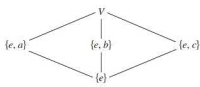
\includegraphics{Klein.png}
\end{figure}
\end{frame}

\begin{frame}{Exercise}
\justifying
Find the subgroups of the group $(Z_4, +_4)$ and construct the lattice diagram for subgroups of $(Z_4, +_4)$. 
\end{frame}

\subsection{Subgroup Tests}

\begin{frame}{Two-Step Subgroup Test}
\begin{definition}
\justifying
Let $H$ be a subset of a group $G$. We say that $H$ is \textbf{closed under taking inverses} if $a^{-1} \in H$ for any $a \in H$ under the induced operation on $H$.
\end{definition}
\pause
\begin{theorem}[Two-Step Subgroup Test]
\justifying
A subset $H$ of a group $G$ is a subgroup of $G$ if and only if
\begin{enumerate}
\justifying
\item $H$ is non-empty,
\item $H$ is closed under the binary operation defined on $G$, and
\item $H$ is closed under taking inverses. 
\end{enumerate}
\end{theorem}
\end{frame}

\begin{frame}{Proof of the Two-Step Subgroup Test}
\begin{proof}
\justifying
Note that associative law holds for any elements in a subset of $G$. Thus, the theorem is proven. 
\end{proof}    
\end{frame}

\begin{frame}{One-Step Subgroup Test}
\begin{theorem}
\justifying
A nonempty subset $H$ of the group $G$ is a subgroup of $G$ under the induced operation on $H$ if and only if $ab^{-1} \in H$ for any $a$ and $b$ in $H$.
\end{theorem}
\pause
\begin{proof}
\justifying
Proof for the necessary part of the theorem clearly follows. Suppose $ab^{-1} \in H$ for all $a, b \in H$. Associative law clearly holds in $H$. Since $H$ is non-empty, there exists an element $x \in H$. Hence $xx^{-1} = e \in H$. Moreover, $ex^{-1} = x^{-1} \in H$. Thus, $H$ is closed under taking inverses. Lastly, suppose that $y \in H$. Therefore, $x\left(y^{-1}\right)^{-1} = xy \in H$ and $H$ is closed under the induced operation from $G$. 
\end{proof}
\end{frame}

\begin{frame}{Finite Subgroup Test}
\begin{theorem}
\justifying
Let $H$ be any non-empty finite subset of a group $G$. If $H$ is closed under the binary operation on $G$, then $H$ is a subgroup of $G$.
\end{theorem}    
\pause
\begin{proof}
\justifying
Suppose that $H$ is closed under the binary operation on $G$. We only need to prove $H$ is closed under taking inverses. If $a = e$, then $a^{-1} = a \in H$. Suppose $a \neq e$. Consider the set $\{a^n: n \in \mathbb{Z}^+\}$. Since $H$ is closed, $a^n \in H$ for each $n \in \mathbb{Z}^+$. By the assumption that $H$ is finite, $a^x = a^y$ for some $x, y \in \mathbb{Z}^+$ such that $x \neq y$. Without loss of generality, we assume that $x > y$. Thus, $a^{x - y} = e$ where $x - y > 1$ since $a \neq e$. It follows that $aa^{x - y - 1} = e$ or $a^{-1} = a^{x - y - 1}$. Observe that $x - y - 1 \geq 1$. Hence, $a^{x - y - 1} \in \{a^n: n \in \mathbb{Z}^+\}$. By the two-step subgroup test, the conclusion follows.
\end{proof}
\end{frame}

\begin{frame}{Exercises}
\begin{enumerate}
\justifying
\item The \textbf{center} $Z(G)$ of a group $G$ is a subset of $G$ containing elements that commute with every element of $G$. That is,
\[
Z(G) := \{a \in G : ag = ga \text{ for all } g \in G\}. 
\]
Prove that the center of a group $G$ is a subgroup of $G$.
\item The \textbf{centralizer} $C(a)$ of an element $a$ of a group $G$ is a subset of $G$ containing elements that commute with $a$. In symbols,
\[
C(a) := \{g \in G : ag = ga\}. 
\]
Prove that the centralizer of $a$ is a subgroup of $G$ for each element $a$ in a group $G$.
\end{enumerate}
\end{frame}

\begin{frame}{Exercises (cont.)}
\begin{enumerate}
\justifying
\item[3. ] Let $G$ be a group and $A$ be a non-empty subset of $G$. The \textbf{normalizer} of $A$ in $G$ is defined as
\[
N_G(A) = \{g \in G: gAg^{-1} = A\}
\]
where $gAg^{-1} = \{gag^{-1}: a \in A\}$. Prove that the normalizer of $A$ in $G$ is a subgroup of $G$.
\item[4. ] Let $H$ and $K$ be subgroups of an abelian group $G$. Show that the set $\{hk: h \in H, k \in K\}$ under the induced operation from $G$ is a subgroup of $G$.
\end{enumerate}
\end{frame}

\begin{frame}{Exercises (cont.)}
\begin{enumerate}
\item[5.] Prove that the intersection $H \cap K$ of two subgroups $H$ and $K$ of a group $G$ is a subgroup of $G$.
\item[6.] Prove that $D$ is a subgroup of $(F, +)$ where $D$ consists of differentiable real-valued functions with domain $\mathbb{R}$. Moreover, show that $\{f \in D: \nicefrac{df}{dx} \text{ is constant}\}$ is a subgroup of $D$.
\end{enumerate}
\end{frame}

\begin{frame}{Additional Notes}
\begin{itemize}
\justifying
\item In the Two-Step Subgroup Test, some references replace the requirement for a subgroup $H$ of a group $G$ to be non-empty by showing that the identity element in $G$ also lies in $H$.  
\item A finite group $G$ cannot be written as a union of two finite proper subgroups of $G$.
\end{itemize}
\end{frame}

\section{Cyclic Groups}

\subsection{Terminologies and Examples}

\begin{frame}{Cyclic Subgroup}
\begin{theorem}
\justifying
Let $G$ be a group. Suppose that $a$ is any element of $G$. The set 
\[
\langle a\rangle := \{a^n : n \in \mathbb{Z}\}
\]
is a subgroup of $G$ under the binary operation on $G$. Furthermore, $\langle a\rangle$ is the smallest subgroup of $G$ that contains $a$, that is, every subgroup containing $a$ contains $\langle a\rangle$. The subgroup $\langle a\rangle$ is called the \textbf{cyclic subgroup generated by $a$}.
\end{theorem}
\end{frame}

\begin{frame}{Proof}
\begin{proof}
\justifying
Note that $e = a^0 \in G$. Suppose that $x, y \in \langle a\rangle$. Then $x = a^m$ and $y = a^n$ for some $m, n \in \mathbb{Z}$. Since 
\[
xy^{-1} = a^m\left(a^n\right)^{-1} = a^{m - n}
\]
and $a^{m-n} \in \langle a\rangle$, $xy^{-1} \in \langle a\rangle$. Thus, $\langle a\rangle$ is a subgroup of $G$.

Now, suppose that $H$ is a subgroup containing $a$. This implies that $a^{-1}$ is also in $H$. By the closure property, $a^n \in H$ for any $n \in \mathbb{Z}$. Therefore, $H$ contains $\langle a\rangle$. 
\end{proof}    
\end{frame}

\begin{frame}{Examples}
\begin{enumerate}
\item What is the cyclic subgroup generated by $3$ in $\mathbb{Z}_{12}$?
\item What is the cyclic subgroup generated by $4$ in $\mathbb{Z}_{18}$?
\item What is the cyclic subgroup generated by $5$ in $U(12)$?
\item What is the cyclic subgroup generated by $5$ in $U(7)$?
\end{enumerate}
\end{frame}

\begin{frame}{Examples}
\begin{enumerate}
\item $\{0, 3, 6, 9\}$ 
\pause
\item $\{0, 2, 4, 6, 8, 10, 12, 14, 16\}$
\pause
\item $\{1, 5\}$
\pause
\item $U(7)$
\end{enumerate}    
\end{frame}

\begin{frame}{Cyclic Group}
\begin{definition}
\justifying
An element $a$ of a group $G$ \textbf{generates} $G$ if $\langle a\rangle = G$. We also say that $a \in G$ is a \textbf{generator} for $G$. 
\end{definition}    
\begin{definition}
\justifying
A group $G$ is said to be \textbf{cyclic} if there exists an element that generates $G$.
\end{definition}
\end{frame}

\begin{frame}{Examples}
\begin{enumerate}
\item The group $\mathbb{Z}_8$ is \_\_\_\_\_\_\_\_\_.
\item The Klein four-group is \_\_\_\_\_\_\_\_\_.
\item The group of units $U(9)$ in $\mathbb{Z}_9$ is \_\_\_\_\_\_\_\_\_.
\end{enumerate}    
\end{frame}

\begin{frame}{Examples}
\begin{enumerate}
\item The group $\mathbb{Z}_8$ is cyclic with generator $1$. The elements $3, 5,$ and $7$ are also generators of the group.
\pause
\item The Klein four-group is not cyclic.
\pause
\item The group of units $U(9)$ in $\mathbb{Z}_9$ is cyclic with generator $2$.
\end{enumerate}    
\end{frame}

\begin{frame}{Subset of Words}
\begin{definition}
\justifying
Let $S$ be a non-empty subset of a group $G$. We define $\langle S\rangle$ as the subset of \textbf{words} made from elements in $S$. In symbols,
\[
\langle S\rangle = \{s_1^{\alpha_1}\cdots s_n^{\alpha_n} : n \in \mathbb{Z}_{\geq 1}, s_i \in S, \alpha_i \in \mathbb{Z}\}.
\]
\end{definition}
\end{frame}

\begin{frame}{Subgroup Generated by a Subset}
\justifying
\begin{theorem}
\justifying
For any non-empty subset $S$ of a group $G$, $\langle S\rangle \leq G$. The subgroup $\langle S\rangle$ is called the \textbf{subgroup generated} by $S$. The elements of $S$ are called the \textbf{generators} of $G$.
\end{theorem}
\end{frame}

\begin{frame}{Group Presentation}
\justifying
We can produce all elements from the set of generators, but the structure of $G$ is determined by the interaction of generators with each other. We call the pair consisting of the generating subset $S$ and the set of relations among these generators as a \textbf{presentation} of the group $G$. We denote a group presentation by
\[
\langle S : \text{ relations}\rangle.
\]

\end{frame}

\begin{frame}{Example}

\begin{enumerate}
\item Create the operation table for the group with presentation
\[
\langle a, b : a^2 = b^2 = (ab)^2 = e\rangle.
\]
\item Let $a = \begin{pmatrix}-1 & 0 \\ 0 & 1\end{pmatrix}$ and $b = \begin{pmatrix}1 & 0 \\ 0 & -1\end{pmatrix}$. Demonstrate that the group generated by $a$ and $b$ in $GL_2(\mathbb{R})$ is an example of a group of order $4$ with presentation
\[
\langle a, b : a^2 = b^2 = (ab)^2 = I\rangle.
\]
\end{enumerate}

\end{frame}

\begin{frame}{Finitely Generated Group}
\begin{definition}
A group is said to be \textbf{finitely generated} if it is generated by a finite subset.
\end{definition}
\end{frame}

\subsection{Properties of Cyclic Groups}

\begin{frame}{Cyclic Groups are Commutative}
\begin{theorem}
\justifying
Every cyclic group is Abelian.
\end{theorem}    
\pause
\begin{proof}
Suppose that $G$ is generated by $a$. Let $x, y \in \langle a\rangle$. Then $x = a^m$ and $y = a^n$ for some $m, n \in \mathbb{Z}$. Observe that
\[
xy = a^ma^n = a^{m + n} = a^{n + m} = a^na^m = yx.
\]
Therefore, $G$ is Abelian.
\end{proof}
\end{frame}

\begin{frame}{Order of a Group Element}
\begin{definition}
\justifying
The \textbf{order} $|a|$ of an element $a$ from a group $G$ is the smallest positive integer $n$ such that $a^n = e$. If no such positive integer exist, then $a$ is said to be of infinite order.
\end{definition}
\end{frame}

\begin{frame}{Examples}
\begin{enumerate}
\item Consider the group $\mathbb{Z}_4$. The order of $3$ is \_\_\_\_\_\_\_\_\_ while the order of $2$ is \_\_\_\_\_\_\_\_\_.
\item The element $5 \in U(7)$ has order \_\_\_\_\_\_\_\_\_.
\item The element $7 \in \mathbb{Z}$ has \_\_\_\_\_\_\_\_\_. 
\end{enumerate}    
\end{frame}

\begin{frame}{Examples}
\begin{enumerate}
\item Consider the group $\mathbb{Z}_4$. The order of $3$ is 4 while the order of $2$ is $2$.
\pause
\item The element $5 \in U(7)$ has order $6$.
\pause
\item The element $7 \in \mathbb{Z}$ has an infinite order. 
\end{enumerate}    
\end{frame}

\begin{frame}{Order of a Cyclic Subgroup}
\begin{lemma}
\justifying
The order of an element $a$ from a group $G$ is the order of the cyclic subgroup generated by $a$. More specifically,
\begin{enumerate}
\justifying
\item if $|\langle a\rangle| = n < \infty$ then $a^n = e$ and $e, a, \dots, a^{n - 1}$ are the distinct elements of $\langle a\rangle$, and
\item if $|\langle a\rangle| = \infty$ then $a^n \neq e$ and $a^x \neq a^y$ for all positive integers $n, x,$ and $y$ such that $x \neq y$.
\end{enumerate}
\end{lemma}
\pause
\begin{proof}
The proof is left as an exercise to the reader.    
\end{proof}
\end{frame}

\begin{frame}{Consequences of the Lemma}
\begin{theorem}
\justifying
Let $G$ be a group. Suppose that $a \in G$ and $k \in \mathbb{Z} - \{0\}$. The following statements hold:
\begin{enumerate}
\justifying
\item If $|a| = \infty$ then $|a^{k}| = \infty$.
\item If $|a| = n < \infty$ then $|a^k| = \nicefrac{n}{\gcd(n, k)}$. 
\end{enumerate}
\end{theorem}  
\begin{corollary}
\justifying
Let $G$ be a group of order $n$. Suppose that $a \in G$ and $k \in \mathbb{Z} - \{0\}$. Then $G = \langle a^k\rangle$ if and only if $\gcd(k, n) = 1$.
\end{corollary}
\end{frame}

\begin{frame}{Alternative Lemma for the Theorem}
\begin{lemma}
Let $G$ be a cyclic group of order $n$. Suppose that $a$ is a generator for $G$. Then $a^k = e$ if and only if $n$ divides $k$.
\end{lemma}
\pause
\begin{proof}
Suppose that $a^k = e$. There exists integers $q, r$ where $0 < r < n$ and
\[
k = nq + r.
\]
Hence, $a^k = a^{nq + r} = a^{nq}a^r$. Since $n$ is the order of $a$, we must have $r = 0$. Thus, $n$ divides $k$. 
On the other hand, if $n$ divides $k$ then $k = nq$ for some integer $q$. Therefore,
\[
a^k = a^{nq} = \left(a^n\right)^q = e^q = e.
\]
\end{proof}
\end{frame}

\begin{frame}{Proof}
\begin{theorem}
\justifying
Let $G$ be a group. Suppose that $a \in G$ and $k \in \mathbb{Z} - \{0\}$. The following statements hold:
\begin{enumerate}
\justifying
\item If $|a| = \infty$ then $|a^{k}| = \infty$.
\item If $|a| = n < \infty$ then $|a^k| = \nicefrac{n}{\gcd(n, k)}$. 
\end{enumerate}
\end{theorem}      
\pause
\begin{proof}
\justifying
The proof for the infinite case is trivial. Suppose that $|a| = n < \infty$. Note that the order of $a^k$ is the smallest integer $m$ such that
\[
\left(a^k\right)^m = e \text{ or } a^{km} = e.
\]
Using the previous lemma, $n$ must divide $km$. If $d = \gcd(n, k)$ then $\nicefrac{n}{d}$ divides $m\left(\nicefrac{k}{d}\right)$. Thus, $\nicefrac{n}{d}$ divides $m$. Therefore, $m = \nicefrac{n}{d}$. 
\end{proof}
\end{frame}

\begin{frame}{Corollaries}
\begin{corollary}
\justifying
Let $G$ be a group of order $n$. Suppose that $a \in G$ and $k \in \mathbb{Z} - \{0\}$. Then $G = \langle a^k\rangle$ if and only if $\gcd(k, n) = 1$.
\end{corollary}
\begin{corollary}
\justifying
The order of an element in a finite cyclic group $G$ divides the order of $G$.
\end{corollary}
\end{frame}

\begin{frame}{Fundamental Theorem of Cyclic Groups}
\begin{theorem}
\justifying
Let $G = \langle a\rangle$ be a cyclic group. Suppose that $|G| = n < \infty$. Every subgroup of a cyclic group is cyclic. Furthermore, the order of any subgroup of $G$ divides $n$. In addition, for each positive integer $k$ dividing $n$, there exists a unique subgroup of $G$ of order $k$. This subgroup is the cyclic group $\langle a^d\rangle$ where $d = \nicefrac{n}{k}$.
\end{theorem}    
\end{frame}

\begin{frame}{Proof}
\begin{proof}
\renewcommand{\qedsymbol}{}
\justifying
Let $G$ be a cyclic group generated by $a$, and $H$ be a subgroup of $G$. If $H$ is a trivial subgroup then the conclusion follows. Suppose that $H$ is non-trivial. This implies that there exists $b \in H$ where $b \neq e$. Note that $b$ is also in $G$. Hence, $b = a^r$ for some nonzero $r \in \mathbb{Z}$. Since $H$ is a subgroup, $a^{-r}$ is also in $H$. This shows that $H$ contains positive powers of $a$ since exactly one of $r$ or $-r$ is positive. From the collection of positive powers of $a$, let $m$ be the smallest element. Such element exists using the Well-Ordered Principle.
\end{proof}
\end{frame}

\begin{frame}{Proof (cont.)}
\begin{proof}
\renewcommand{\qedsymbol}{}
\justifying
We claim that $a^m$ is a generator for $H$. Consider $h \in H \subset G$. We can also write $h$ as $a^k$ for some $k \in \mathbb{Z}$. By the Division Algorithm, there exists integers $q$ and $r$ such that $k = mq + r$ where $0 \leq r < m$. Observe that
\[
a^k = a^{mq + r} = a^{mq}a^r = \left(a^m\right)^qa^r.
\]
Hence, $a^r = a^k\left(a^m\right)^{-q}$ and $a^r \in H$. Note that $m$ is the smallest positive element such that $a^m \in H$. Thus, $r = 0$ and
\[
h = \left(a^m\right)^q.
\]
Therefore, $H$ is cyclic with generator $a^m$.
\end{proof}    
\end{frame}

\begin{frame}{Proof (cont.)}
\begin{proof}
\renewcommand{\qedsymbol}{}
\justifying
Let $H$ be a subgroup of $G$. Then $H$ is cyclic and $H = \langle a^m\rangle$ where $m$ divides $n$. Also $H$ satisfies 
\[
|H| = \left|\langle a^m\rangle\right| = \dfrac{n}{\gcd(n, m)} = \dfrac{n}{m}. 
\]
Hence, the order of any subgroup of $G$ divides $n$. Now, let $k$ be a divisor of $n$. Note that 
\[
\left|\left\langle a^{\nicefrac{n}{k}}\right\rangle\right| = \dfrac{n}{\gcd\left(n, \frac{n}{k}\right)} = \dfrac{n}{\nicefrac{n}{k}} = k.
\]
This shows that $G$ has a subgroup of order $k$. 
\end{proof}    
\end{frame}

\begin{frame}{Proof (cont.)}
\begin{proof}
\justifying
Suppose that $K$ is another subgroup of order $k$. Then $K$ must also be cyclic and has generator $a^s$ where $s$ divides $n$. Also, 
\[
k = |K| = |a^s| = \dfrac{n}{\gcd(n, s)} = \dfrac{n}{s}.
\]
Therefore, $s = \dfrac{n}{k}$.
\end{proof}    
\end{frame}

\begin{frame}{Corollary of an Important Theorem}
\begin{corollary}
\justifying
Let $G$ be a finite cyclic group and $H \leq G$. The order $|H|$ of $H$ must divide that $|G|$ of $G$. In other words, $|G|$ is a multiple of $|H|$.
\end{corollary}     
\begin{corollary}
\justifying
For each integer $k$ dividing $n$, the set $\left\langle \frac{n}{k}\right\rangle$ is the unique subgroup of $\mathbb{Z}_n$ with order $k$. Moreover, these are only the subgroups of $\mathbb{Z}_n$. 
\end{corollary}   
\end{frame}

\begin{frame}{Other Corollaries}
\begin{corollary}
\justifying
Let $d$ be a divisor of $n$. The number of elements of order $d$ in a cyclic group of order $n$ is $\phi(d)$, the number of positive integers less than $d$ relatively prime to $d$.
\end{corollary}   
\begin{corollary}
\justifying
In a finite group, the number of elements of order $d$ is a multiple of $\phi(d)$.
\end{corollary}   
\end{frame}

\begin{frame}{Exercises}
\begin{enumerate}
\justifying
\item Find all generators and draw the lattice diagram of subgroups for $\mathbb{Z}_{16}$, $\mathbb{Z}_{28}$, $U(18)$, and $U(24)$.
\item Suppose that $a$ and $b$ are elements of a finite group such that $ab = ba$. Show that the order $|ab|$ of $ab$ divides the product $|a||b|$ of the orders of $a$ and $b$. In addition, show that $|ab| = |a||b|$ if and only if $\gcd(|a|, |b|) = 1$.
\item Prove that a group of order $3$ is always cyclic.
\end{enumerate}    
\end{frame}

\section{Examples of Non-Abelian Groups}

\subsection{Symmetric Group}

\begin{frame}{Permutation}
\begin{definition}
\justifying
A \textbf{permutation} of a set $A$ is a function $\phi: A \rightarrow A$ from a set into itself that is both one-to-one and onto. 
\end{definition}
\pause
\begin{definition}[Restated]
\justifying
A \textbf{permutation} of a set $A$ is a bijective function from $A$ onto itself.
\end{definition}
\end{frame}

\begin{frame}{Permutation Group}
\justifying
\begin{theorem}
\justifying
The collection of all permutations of a set $A$ into itself is a group under function composition.
\end{theorem}
\pause
\begin{proof}
\justifying
The proof follows from the definition and properties of a bijective function.
\end{proof}
\end{frame}

\begin{frame}{Symmetric Group on $n$ Letters}
\justifying
The collection of all permutations on a set $A$ under function composition forms a group called the \textbf{symmetric group} on $A$. By letting $A$ be the set $Q_n := \{1, \dots, n\}$, we call the symmetric group $S_n$ on $Q_n$ as the \textbf{symmetric group on $\boldsymbol{n}$ letters}.    
\end{frame}

\begin{frame}{Example}
What are the elements of the symmetric group $S_3$ on $3$ letters? \newline\newline
\pause
Consider a function from the set $\{1, 2, 3\}$ onto $\{1, 2, 3\}$. The only possible bijective functions are those functions whose mappings are given by:
\begin{enumerate}
\item $1 \mapsto 1, 2 \mapsto 2$, and $3 \mapsto 3$,
\item $1 \mapsto 1, 2 \mapsto 3$, and $3 \mapsto 2$,
\item $1 \mapsto 3, 2 \mapsto 2$, and $3 \mapsto 1$,
\item $1 \mapsto 2, 2 \mapsto 1$, and $3 \mapsto 3$,
\item $1 \mapsto 2, 2 \mapsto 3$, and $3 \mapsto 1$, and
\item $1 \mapsto 3, 2 \mapsto 1$, and $3 \mapsto 2$.
\end{enumerate}
\end{frame}

\begin{frame}{Two-Line Notation}
A permutation $\sigma$ on $Q_n$ can be expressed in the two-line notation shown below
\[
\begin{pmatrix}
1 & 2 & \cdots & n \\
\sigma(1) & \sigma(2) & \cdots & \sigma(n)
\end{pmatrix}.
\]
\pause
With this notation, the inverse of a permutation is given by
\[
\begin{pmatrix}
\sigma(1) & \sigma(2) & \cdots & \sigma(n) \\
1 & 2 & \cdots & n 
\end{pmatrix}.
\]
\end{frame}

\begin{frame}{Example (Revisited)}
\justifying
Using the two-line notation, the elements of $S_3$ are
\begin{align*}
&\begin{pmatrix} 1 & 2 & 3 \\ 1 & 2 & 3 \end{pmatrix}, \begin{pmatrix} 1 & 2 & 3 \\ 1 & 3 & 2 \end{pmatrix},
\begin{pmatrix} 1 & 2 & 3 \\ 3 & 2 & 1 \end{pmatrix}, \\
&\begin{pmatrix} 1 & 2 & 3 \\ 2 & 1 & 3 \end{pmatrix},
\begin{pmatrix} 1 & 2 & 3 \\ 2 & 3 & 1 \end{pmatrix}, \text{ and }
\begin{pmatrix} 1 & 2 & 3 \\ 3 & 1 & 2 \end{pmatrix}.
\end{align*}
\pause
Now, we use the notation to easily compute for the composition of permutations. Let 
\[
f = \begin{pmatrix} 1 & 2 & 3 \\ 1 & 3 & 2 \end{pmatrix} \text{ and } g = \begin{pmatrix} 1 & 2 & 3 \\ 3 & 2 & 1 \end{pmatrix}.
\]
We compute for $f \circ g$. Note that finding composition of two permutations shall be read from right to left.
\end{frame}

\begin{frame}{Cycle Notation}
\justifying
Given the permutation $\sigma = \begin{pmatrix} 1 & 2 & 3 & 4 & 5 & 6 \\ 2 & 1 & 4 & 6 & 5 & 3 \end{pmatrix}$ on $Q_6$, it can be expressed simply as
\[
(1 \ 2)(3 \ 4 \ 6)(5)
\]
where the objects $(a_1 \ a_2 \ \dots \ a_{n - 1} \ a_n)$, referred to as \textbf{cycles of length $\boldsymbol{n}$} or \textbf{$\boldsymbol{n}$-cycles}, satisfies $\sigma(a_1) = a_2, \dots$, $\sigma\left(a_{n - 1}\right) = a_n$, and $\sigma(a_n) = a_1$. The product of cycles is called the \textbf{cycle decomposition} of $\sigma$.
\end{frame}

\begin{frame}{Cycle Decomposition Algorithm}
    \justifying
    \begin{enumerate}
        \justifying
        \item Select the smallest element $a$ which has not appeared in a previous cycle.
        \item Find the image $b$ of the element to obtain an initial cycle $(a \ b$. Repeat this step until we reach an element $k$ which is mapped to $a$. 
        \item We close the cycle with a right parenthesis. For instance, we have the cycle $(a \ b \ \dots k)$.
        \item Repeat the first step until all elements of $S_n$ are considered.
        \item Remove all cycles of length one (1).
    \end{enumerate}
\end{frame}

\begin{frame}{Examples}
\begin{enumerate}
\justifying
\item Consider the permutations in $S_6$ given by
\[
\sigma = \begin{pmatrix}
1 & 2 & 3 & 4 & 5 & 6 \\
2 & 5 & 6 & 1 & 4 & 3
\end{pmatrix} \text{ and }
\delta = \begin{pmatrix}
1 & 2 & 3 & 4 & 5 & 6 \\
1 & 4 & 2 & 6 & 5 & 3
\end{pmatrix}.
\]
What are $\sigma \circ \delta$ and $\delta \circ \sigma$?
\item Evaluate all powers of the permutation $\sigma \in S_5$ given by
\[
\begin{pmatrix} 1 & 2 & 3 & 4 & 5 \\ 5 & 2 & 1 & 4 & 3 \end{pmatrix}.
\]
\end{enumerate}    
\end{frame}

\begin{frame}{Remarks}
\begin{itemize}
\item For all integers $n \geq 3$, the symmetric group on $n$ letters is non-Abelian.
\item For any cycle $(a_1 \ a_2 \ \dots \ \ a_n )$ of length $n$, 
\[
(a_1 \ a_2 \ \dots \ \ a_n ) = (a_2 \ \dots \ \ a_n \ a_1 ) = \cdots = (\dots \ a_n \ a_1 \ a_2).
\]
\end{itemize}    
\end{frame}

\begin{frame}{Disjoint Cycles}
\justifying
Cycles that have no entries in common are said to be \textbf{disjoint}.    
\newline\newline
\pause
For instance, the cycles $(1 \ 4 \ 7)$ and $(6 \ 5)$ are disjoint while $(2 \ 5 \ 3)$ and $(3 \ 7)$ are not disjoint.
\newline\newline
\pause
The inverse of a permutation $(a_1 \ \dots \ a_n)(b_1 \ \dots \ b_k)\cdots$, where the cycles are pairwise disjoint, is then given by
\[
\cdots(b_k \ \dots \ b_1)(a_n \ \dots \ a_1).
\]
\end{frame}

\begin{frame}{Examples}
\begin{enumerate}
\item Write the permutation $\begin{pmatrix} 1 & 2 & 3 & 4 & 5 & 6 \\ 5 & 3 & 1 & 6 & 2 & 4 \end{pmatrix}$ and its inverse using disjoint cycles.
\item Consider the permutations in $S_7$ given by $\sigma = (1 \ 3 \ 4)(5 \ 6 \ 2)$ and $\delta = (2 \ 4)(3 \ 6)$. Compute for $\sigma\delta$ and $\delta\sigma$.
\end{enumerate}    
\end{frame}

\subsubsection{Properties of Symmetric Groups}

\begin{frame}{Cycle Decomposition of a Permutation}
\begin{theorem}
Every permutation of a finite set can be written as a cycle or as a product of disjoint cycles.
\end{theorem}
\pause
\begin{proof}
The proof is left as an exercise to the reader.    
\end{proof}
\end{frame}

\begin{frame}{Disjoint Cycles Commute}
\begin{theorem}
Given any pair of disjoint cycles $\sigma$ and $\delta$, we must have $\sigma\delta = \delta\sigma$.
\end{theorem}    
\pause
\begin{proof}
\justifying
Let $x$ be an entry in $\sigma$. Then $\sigma(x)$ is an entry in $\sigma$ and $\delta(y) = y$ for all entries $y$ in $\sigma$. Hence, $\sigma(\delta(x)) = \sigma(x) = \delta(\sigma(x))$. Similar arguments follow when $x$ is an entry in $\delta$.
\end{proof}
\end{frame}

\begin{frame}{Order of a Cycle}
\begin{lemma}
The order of a $k$-cycle is $k$. 
\end{lemma}
\pause
\begin{proof}
Let $\sigma = (a_1 \ a_2 \ \dots \ a_k)$ be a $k$-cycle. Note that $\sigma(a_i) = a_{i + 1}$. Hence, $\sigma^n(a_i) = a_{i + n}$ where $i + n$ is taken modulo $k$. This shows that $\sigma^k(a_i) = a_i$ and $\sigma^j(a_1) \neq a_1$ for $1 \leq j \leq k-1$. Therefore, $\sigma^j \neq (1)$ whenever $1 \leq j \leq k -1$ and $|\sigma| = k$.
\end{proof}
\end{frame}

\begin{frame}{Order of a Permutation}
\begin{theorem}
\justifying
The order a permutations is the least common multiple of the lengths of the cycles in its cycle decomposition.    
\end{theorem}
\pause
\begin{proof}
\justifying
Let $\alpha = \alpha_1\dots\alpha_n$ be a cycle decomposition where the length of $\alpha_i$ is $l_i$. Suppose that $k$ is the order of $\alpha$ and $l$ be the least common multiple of $l_1$, \dots, and $l_n$. Then $\alpha^k = \alpha_1^k\cdots\alpha_n^k = (1)$ because disjoint cycles commute. It follows that $\alpha_i^k = (1)$ for all $i$ since $\alpha_i^k$ are disjoint. Thus, each $l_i$ divides $k$ which implies that $l$ divides $k$. Moreover, $\alpha^l = (1)$ since $\alpha_i^{l_i} = (1)$. This means that $k$ divides $l$. Therefore, $k = l$.
\end{proof}
\end{frame}

\begin{frame}{Examples}
Find the order of the following permutations.
\begin{enumerate}
    \item $(1 \ 3 \ 4)(2 \ 5)$
    \item $(1 \ 7 \ 3)(4 \ 8)(2 \ 5 \ 6 \ 9)$
    \item $(1 \ 5 \ 4 \ 2)(2 \ 5 \ 7 \ 9)$
\end{enumerate}
\end{frame}

\begin{frame}{Transposition}
\begin{definition}
\justifying
A cycle of length 2 is called a \textbf{transposition}.
\end{definition} 
\pause
\begin{theorem}
\justifying
Every permutation of a finite set containing at least two elements is a product of $2$-cycles.
\end{theorem}
\pause
\begin{proof}
\justifying
The proof follows from the fact that any cycle $(a_1 \ a_2 \ \dots \ a_k)$ can be written as $(a_1 \ a_k)\dots(a_1 \ a_3)(a_1 \ a_2)$.   
\end{proof}
\end{frame}

\begin{frame}{Even and Odd Permutations}
\begin{lemma}
If $\sigma_1\dots\sigma_k = (1)$ then $k$ must be even. 
\end{lemma}
\pause
\begin{proof}
The proof is left as an exercise to the reader.    
\end{proof}
\end{frame}

\begin{frame}{Unique Parity}
\begin{theorem}
\justifying
No permutation in $S_n$ can be expressed both as a product of an even number of transpositions and as a product of an odd number of transpositions.
\end{theorem}
\pause
\begin{proof}
Let $\alpha = \alpha_1\dots\alpha_k$ and $\beta = \beta_1\dots\beta_j$. If $\alpha = \beta$ then 
\[
\alpha_1\dots\alpha_k\beta_j^{-1}\dots\beta_1^{-1} = \alpha_1\dots\alpha_k\beta_j\dots\beta_1 = (1).
\]
Thus, $s + r$ must be even. Therefore, $s$ and $r$ must be both odd or both even.
\end{proof}
\end{frame}

\begin{frame}{Parity of Permutations}
\begin{definition}
\justifying
A permutation of a finite set is \textbf{even} or \textbf{odd} if it can be written as a product of an even or odd number of transpositions, respectively.
\end{definition}
\end{frame}

\begin{frame}{Inversion}
	\justifying
	\begin{definition}
	\justifying
	Let $n$ be an integer with $n \geq 2$. Define $T_n$ as the set of ordered pairs given by
	\[
	T_n = \{(i, j) \in Q_n^2 : i < j\}.
	\]
	The number of \textit{inversions} of $\sigma \in S_n$ is the number
	\[
	\text{inv}(\sigma) = \left|\{(i, j) \in T_n : \sigma(i) > \sigma(j)\}\right|.
	\]
	\end{definition}
	Observe that 
	\[
	|T_n| = \sum_{i = 1}^n(n - i) = n(n - 1) - \sum_{i = 1}^ni = \dfrac{n(n-1)}{2}.
	\]
\end{frame}

\begin{frame}{Example}
\justifying
Consider the permutation $\sigma = (1 \ 3 \ 2)(4 \ 5)$ in $S_5$. To find $\text{inv}(\sigma)$, we must find pairs $(i, j) \in Q_5^2$ such that $\sigma(i) > \sigma(j)$. These are the pairs 
\[
(1, 2), (1, 3), \text{ and } (4, 5).
\]
Hence, $\text{inv}(\sigma) = 3$.
\end{frame}

\begin{frame}{Parity}
\begin{theorem}
\justifying
A permutation $\sigma \in S_n$ is even (odd) if and only if $\text{inv}(\sigma)$ is an even (odd) integer.
\end{theorem}
\begin{proof}
The proof is left as an exercise.
\end{proof}
\end{frame}

\subsubsection{Alternating Group}

\begin{frame}{Alternating Group on $n$ Letters}
\begin{theorem}
\justifying
Let $n \geq 2$ be an integer. The collection of all even permutations of $\{1, 2, \dots, n\}$ forms a subgroup of order $\nicefrac{n!}{2}$ of the symmetric group $S_n$. This subgroup is called the \textbf{alternating group on $\boldsymbol{n}$ letters}.      
\end{theorem}
\pause
\begin{proof}
\justifying
Consider the function $f: A_n \rightarrow S_n - A_n$ defined by $f(\sigma) = \alpha\sigma$ where $\alpha$ is a fixed element of $S_n - A_n$. We claim that $f$ is bijective. Suppose that $f(\sigma) = f(\beta)$. Then $\alpha\sigma = \alpha\beta$. Hence, $\sigma = \beta$ and $f$ is one-to-one. Now, we consider $\delta \in S_n - A_n$. Then $\alpha^{-1}\delta$ is an even permutation and $f(\alpha^{-1}\delta) = \delta$. Thus, $f$ is onto. Therefore, $f$ is bijective and $|A_n| = |S_n - A_n| = \frac{n!}{2}$.
\end{proof} 
\end{frame}

\begin{frame}{Exercises}
\begin{enumerate}
\justifying
\item What are the possible orders for the elements of $S_5$?
\item Let $H = \{\beta \in S_5: \beta(1) = 1 \text{ and } \beta(3) = 3\}$. Prove that $H$ is a subgroup of $S_5$. Find the order of $H$.
\item Prove that for any permutation $\sigma$, $\sigma\tau\sigma^{-1}$ is a transposition if and only if $\tau$ is a transposition.
\end{enumerate}
\end{frame}

\begin{frame}{Additional Notes}
\begin{itemize}
\item Symmetric groups on $n$ letters are also called \textbf{symmetric groups of degree $\boldsymbol{n}$}.
\item Any subgroup of a symmetric group of a set is called a \textbf{permutation group}.
\item The product of all cycles relating to a permutation $\sigma$ is called the \textbf{cycle decomposition} of $\sigma$.
\end{itemize}    
\end{frame}

\subsection{Dihedral Group}

\begin{frame}{Elements of the Dihedral Set}
The elements of $D_{2n}$ are composed of
\begin{itemize}
    \item $n$ rotations, and
    \item $n$ reflection symmetries.
\end{itemize}
These rotation and reflection symmetries can be written in terms of permutations.
\end{frame}

\begin{frame}{Dihedral Symmetries of the Square}
For instance, the elements of $D_{8}$ are subsets of $S_4$ given by the rotations
\begin{enumerate}
\begin{multicols}{2}
    \item $(1)$
    \item $(1 \ 2 \ 3 \ 4)$
    \item $(1 \ 3)(2 \ 4)$ and
    \item $(1 \ 4 \ 3 \ 2)$,
    \end{multicols}
\end{enumerate}
and the reflection symmetries
\begin{enumerate}
\begin{multicols}{2}
    \item $(1 \ 2)(3 \ 4)$
    \item $(2 \ 4)$
    \item $(1 \ 3)$ and
    \item $(1 \ 4) (2 \ 3)$.
    \end{multicols}
\end{enumerate}
\end{frame}

\begin{frame}{Dihedral Group}
\begin{theorem}
\justifying
For any $n \geq 3$, $\left(D_{2n}, \circ\right)$ is a group under function composition.
\end{theorem}
\pause
\begin{theorem}
The proof follows from the definition of a symmetry.    
\end{theorem}
\end{frame}

\begin{frame}{Dihedral Group}
\begin{definition}
\justifying
Let $n \geq 3$. The \textbf{dihedral group} $D_{2n}$ of order $2n$ is the set $D_{2n}$ under the function composition.
\end{definition}
\pause
\begin{definition}[Restated]
\justifying
The \textbf{dihedral group} $D_{2n}$ of order $2n$, where $n \geq 3$, is the group consisting of all rigid motions of a regular polygon with $n$ sides under the function composition. 
\end{definition}    
\end{frame}

\begin{frame}{Dihedral Group (cont.)}    
\begin{lemma}
\justifying
The dihedral group $D_{2n}$ can be expressed as 
\[
\{1, \rho, \rho^2, \dots, \rho^{n-1}, \mu\rho, \mu\rho^2, \dots, \mu\rho^{n-1}\}
\]
where $\rho$ is the clockwise rotation about the origin through $\nicefrac{2\pi}{n}$ radians and $\mu$ is the reflection about the line of symmetry passing through vertex $1$ and the origin. 
\end{lemma}
\pause
\begin{proof}
The proof is left as an exercise to the reader.
\end{proof}
\end{frame}

\begin{frame}{Properties of Dihedral Groups}
\begin{theorem}
\justifying
Let $D_{2n}$ be the dihedral group of order $2n$. The following statements hold:
\begin{enumerate}
\item The order of $\rho$ and $\mu$ is $n$ and 2 respectively.
\item For any integers $i$ and $j$, $\rho^{i}\rho^j = \rho^{i+j}$.
\item For any $1 \leq i \leq n - 1$, $\mu \neq \rho^i$.
\item For $0 \leq i \leq n$, $\rho^i\mu = \mu\rho^{-i}$ holds.
\end{enumerate}
\end{theorem}
\pause
\begin{proof}
The proof is left as an exercise to the reader.
\end{proof}
\end{frame}

\begin{frame}{Additional Notes}
\begin{itemize}
\justifying
\item The dihedral group of order $2n$ is also called the \textbf{$\boldsymbol{n}$th dihedral group}.
\end{itemize}    
\end{frame}

\section{Cosets}

\subsection{Equivalence Relation on Groups}

\begin{frame}{Group Partition}
\begin{theorem}
Let $H$ be a subgroup of a group $G$. The relation $\sim_L$ defined on $G$ where
\[
a \sim_L b \text{ if and only if } ab^{-1} \in H
\]
is an equivalence relation on $G$.
\end{theorem}
\pause
Observe that the equivalence class $[a]$ containing $a$ can be written as
\begin{align*}
[a] &= \{b \in H: b \sim_L a\} = \{b \in H: ba^{-1} \in H\} \\
&= \{b \in H: ba^{-1} = h \text{ for some } h \in H\} \\
&=  \{b \in H: b = ha \text{ for some } h \in H\} \\
&=  \{ha: h \in H\}.
\end{align*}
\end{frame}

\subsection{Definition}

\begin{frame}{Coset}
\begin{definition}
\justifying
Let $H$ be a subgroup of a group $G$. The subsets $aH = \{ah: h \in H\}$ and $Ha = \{ha: h \in H\}$ of $G$ are respectively called the \textbf{left coset} and \textbf{right coset} of $H$ containing $a \in G$. Any element of a coset is called a \textbf{representative} of a coset.
\end{definition}    
\end{frame}

\begin{frame}{Examples}
\begin{enumerate}
    \item Consider the subgroup $\{0, 3\}$ of $\mathbb{Z}_6$. Find the following cosets $0H, 1H, 4H, 5H, H1$, and $H2$.
    \item Consider the subgroup $H = \{(1), (1 \ 2 \ 3), (1 \ 3 \ 2)\}$ of $S_3$. Find all the left and right cosets of $K$.
    \item Consider the subgroup $K = \{(1), (1 \ 2)\}$ of $S_3$. Find all the left and right cosets of $K$.
\end{enumerate}    
\end{frame}

\begin{frame}{Equivalent Conditions}
\begin{lemma}
Let $H$ be a subgroup of a group $G$. Suppose that $g_1, g_2 \in G$. The following conditions are equivalent:
\begin{enumerate}
    \item $g_1H = g_2H$
    \item $Hg_1^{-1} = Hg_2^{-1}$
    \item $g_1H \subset g_2H$
    \item $g_2 \in g_1H$
    \item $g_1^{-1}g_2 \in H$
\end{enumerate}
\end{lemma}
\end{frame}

\begin{frame}{Cardinality of Left and Right Cosets}
\begin{theorem}
\justifying
Let $H$ be a subgroup of a group $G$. The number of left cosets of $H$ in $G$ is the same as the number of right cosets of $H$ in $G$.
\end{theorem}    
\end{frame}

\begin{frame}{Index of a Subgroup}
\begin{definition}
\justifying
Let $H$ be a subgroup of a (possibly infinite) group $G$. The number of left cosets of $H$ in $G$ is the \textbf{index} of $H$ in $G$, denoted by $(G:H)$.
\end{definition}
\end{frame}

\begin{frame}{Cardinality of $G$ and $gH$}
\begin{lemma}
\justifying
Let $H$ be a subgroup of a group $G$. The cardinality of $H$ is equal to the cardinality of any left coset $gH$ of $H$ in $G$. 
\end{lemma}
\end{frame}

\begin{frame}{Theorem of Lagrange}
\begin{theorem}
Let $H$ be a subgroup of a finite group $G$. Then the order of $H$ divides the order of $G$. In particular, 
\[
|G| = \dfrac{(G:H)}{|H|}.
\]
\end{theorem}
\end{frame}

\begin{frame}{Groups of Prime Order}
\begin{corollary}
Every group $G$ of prime order is cyclic. In addition, any element of $G$ is a generator for $G$.
\end{corollary}    
\end{frame}

\begin{frame}{Corollary}
\begin{corollary}
The order of an element in a finite group $G$ divides the order of $G$.    
\end{corollary}
\begin{corollary}
\justifying
    If $G$ is a group of prime order $p$, then $G$ is cyclic. Specifically, $G$ is isomorphic to $\mathbb{Z}_p$.
\end{corollary}
\end{frame}

\begin{frame}{Corollary}
\begin{corollary}
\justifying
Let $H$ and $K$ be subgroups of a group $G$ such that $K \leq H \leq G$. Suppose that $(H:K)$ and $(G:H)$ are both finite. Thus, $(G:K)$ is finite and $(G:K) = (G:H)(H:K)$.
\end{corollary}    
\end{frame}

\begin{frame}{Exercises}
    \begin{enumerate}
    \justifying
        \item Suppose that $(G:H)=2$. If $a$ and $b$ are not in $H$, then $ab \in H$.
        \item If $(G:H) = 2$, then $gH = Hg$.
        \item Let $H$ and $K$ be subgroups of a group $G$. Prove that $gH \cap gK$ is a coset of $H \cap K$ in $G$.
    \end{enumerate}
\end{frame}

\section{Group Isomorphism}

\subsection{Cayley's Theorem}

\begin{frame}{Isomorphism}
\begin{definition}
\justifying
Let $(G, *)$ and $(H, \star)$ be groups, and $f : G \rightarrow H$. We say that $f$ is a \textbf{group isomorphism} if $f$ is a bijective homomorphism, that is,
\begin{enumerate}
\justifying
\item The function $f$ is one-to-one and maps onto $H$.
\item For all $a, b \in G$, $f(a * b) = f(a) \star f(b)$.
\end{enumerate}
We say that $(G, *)$ is \textbf{isomorphic} to $(H, \star)$ if there exists an isomorphism between $(G, *)$ and $(H, \star)$. We denote these statement by $G \cong H$.
\end{definition}    
\end{frame}

\begin{frame}{"Up to an Isomorphism"}
\justifying
Consider a group $(G, *)$ with three elements say $\{e, a, b\}$. Since a group needs an identity element, we assume that the identity element is $e$. We can construct a Cayley table as follows:
\[
\begin{tabular}{c|c|c|c}
$\ast$ & e & a & b  \\
\hline
e & e & a & b  \\
\hline
a & a & b & e  \\
\hline
b & b & e & a  \\
\end{tabular}.    
\]
The Cayley table of another group with three elements must be similar to the previous table. Hence, up to an isomorphism, there is a unique group of order 3.
\end{frame}

\begin{frame}{Examples}
\begin{enumerate}
\justifying
\item The additive group $(\mathbb{R}, +)$ of real numbers is isomorphic to multiplicative group $(\mathbb{R}, \cdot)$ of real numbers.
\item The groups $U(8)$ and $U(12)$ are isomorphic.
\item The groups $\mathbb{Z}_8$ and $\mathbb{Z}_{12}$ are not isomorphic.
\item The groups $\mathbb{Z}_6$ and $S_3$ are not isomorphic.
\end{enumerate}    
\end{frame}

\begin{frame}{Properties of an Isomorphism}
\begin{lemma}
\justifying
Let $f: G \rightarrow H$ be a group isomorphism between $(G, *)$ and $(H, \star)$. Then $f^{-1}: H \rightarrow G$ is also a group isomorphism and $|G| = |H|$.
\end{lemma}
\pause
\begin{proof}
The proof is left as an exercise to the reader.
\end{proof}
\end{frame}

\begin{frame}
\begin{theorem}
The isomorphism of groups determines an equivalence relation on the class of all groups.    
\end{theorem}
\pause
\begin{proof}
The proof is left as an exercise to the reader.    
\end{proof}
\end{frame}

\begin{frame}{Properties of an Isomorphism (cont.)}
\begin{theorem}
\justifying
Let $f: G \rightarrow H$ be a group isomorphism. Then the following statements hold:
\begin{enumerate}
    \item $G$ has generator $a$ if and only if $H$ has generator $\phi(a)$.
    \item The elements $a$ in $G$ and $\phi(a)$ in $H$ have the same order.
    \item If $G$ is Abelian, then $H$ is Abelian.
    \item If $G$ has a subgroup of order $n$, then $H$ has a subgroup of order $n$.
\end{enumerate}
\end{theorem}
\end{frame}

\begin{frame}{Proving Two Groups are Not Isomorphic}
    \justifying
    Let $G$ and $H$ be groups. Then $G$ is not isomorphic to $H$ whenever
    \begin{enumerate}
        \item $|G| \neq |H|$,
        \item $G$ ($H$) is Abelian and $H$ ($G$) is non-Abelian,
        \item the largest order of any element in $G$ is not equal to the largest order of any element in $H$, or
        \item the number of elements of some specific order in $G$ is not the same as the number of elements of the same order in $H$.
    \end{enumerate}
\end{frame}

\begin{frame}{Examples}
    \justifying
    \begin{enumerate}
        \item The groups $\mathbb{Z}_{12}$ and $D_{12}$ are not isomoprhic.
        \item The group $\mathbb{Q}$ of rational numbers under addition is not isomorphic to the group $\mathbb{Q}^*$ of nonzero rational numbers under multiplication.
    \end{enumerate}
\end{frame}

\begin{frame}{Characterizing Cyclic Groups}
\begin{theorem}
\justifying
Let $G$ be a cyclic group. If the order of $G$ is infinite, then $G$ is isomorphic to $(\mathbb{Z}, +)$. However, If $G$ has finite order $n$ then $G$ is isomorphic to $(\mathbb{Z}_n, +_n)$. 
\end{theorem}
\pause
\begin{proof}
The proof is left as an exercise to the reader.
\end{proof}
\end{frame}

\begin{frame}{Examples}
\begin{enumerate}
\justifying
\item The groups $(\mathbb{Z}, +)$ and $(2\mathbb{Z}, +)$ are isomorphic.
\item The groups $(\mathbb{Z}_n, +_n)$ and $\left(\dfrac{\mathbb{Z}}{n\mathbb{Z}}, \oplus\right)$ are isomorphic.
\end{enumerate}
\end{frame}

\begin{frame}{Cayley's Theorem}
\begin{theorem}
\justifying
Every group is isomorphic to a group of permutations.
\end{theorem}
\pause
\begin{proof}
The proof is left as an exercise to the reader.    
\end{proof}
\end{frame}

\begin{frame}{Left and Right Regular Representation}
\begin{definition}
\justifying
Let $G$ be a group. The function $\phi: G \rightarrow S_G$, where $S_G := \{\lambda_g: g \in G\}$ and $\lambda_g(x) = gx$ for all $x \in G$ is called the \textbf{left regular representation} of $G$. Moreover, the map $\tau: G \rightarrow S_G$ given by $\tau(x) = \sigma_{x^{-1}}$ where $\sigma_g = xg$ for all $x \in G$ is called the \textbf{right regular representation} of $G$.
\end{definition}    
\end{frame}

\subsection{Automorphism}

\begin{frame}{Automorphism}
    \begin{definition}
    \justifying
        An isomorphism from a group $G$ onto itself is called an \textbf{automorphism} of $G$.
    \end{definition}
\end{frame}

\subsubsection{Inner Automorphism}

\begin{frame}{Inner Automorphism}
    \begin{theorem}
        \justifying
        Let $G$ be a group, and $a$ be a fixed element of $G$. The function $\phi_a$ defined by $\phi_a(x) = axa^{-1}$ for all $x$ in $G$ is an automorphism, called the \textbf{inner automorphism} of $G$ induced by $a$.  
    \end{theorem}
    \pause
    \begin{proof}
        The proof is left as an exercise to the reader.    
    \end{proof}
\end{frame}

\begin{frame}{Examples}
    \justifying
    \begin{enumerate}
        \item The function $\phi: \mathbb{R}^2 \to \mathbb{R}^2$ defined by $\phi(a, b) = (b, a)$ is an automorphism of $\mathbb{R}^2$ under componentwise addition.
    \end{enumerate}
\end{frame}

\begin{frame}{Examples}
    \justifying
    \begin{enumerate}
    \justifying
    \item Suppose that $\phi: \mathbb{Z}_{20} \to \mathbb{Z}_{20}$ is an automorphism and $\phi(5) = 5$. What are the possibilities of $\phi(x)$?
        \item Compute $\text{Aut}(\mathbb{Z}_{10})$. 
    \end{enumerate}
\end{frame}

\begin{frame}{Group Isomorphisms}
    \begin{theorem}
        \justifying
        The set $\text{Aut}(G)$ of automorphism of a group $G$ and the set $\text{Inn}(G)$ of inner automorphisms of $G$ are groups under the operation of function composition.
    \end{theorem}
    \pause
    \begin{proof}
        The proof is left as an exercise to the reader.
    \end{proof}
\end{frame}

\begin{frame}{Isomorphism}
    \begin{theorem}
        \justifying
        For every positive integer $n$, $\text{Aut}(\mathbb{Z}_n)$ is isomorphic to $U(n)$.
    \end{theorem}
    \pause
    \begin{proof}
        The proof is left as an exercise to the reader.    
    \end{proof}
\end{frame}

\begin{frame}{Exercises}
    \justifying
    \begin{enumerate}
        \justifying
        \item Suppose that a group $G$ is isomoprhic to a group $H$. Show that $\text{Aut}(G)$ is isomorphic to $\text{Aut}(H)$. 
    \end{enumerate}
\end{frame}

\subsection{Direct Product}

\subsubsection{External Direct Product}

\begin{frame}{Groups from Cartesian Products}
    \begin{theorem}
        \justifying
        Let $G$ and $H$ be groups. The set $G \times H$ is a group under the operation
        \[(g_1,h_1)(g_2, h_2) = (g_1g_2, h_1h_2)\]
        where $g_1, g_2 \in G$ and $h_1, h_2 \in H$. The group is called the \textbf{external direct product} of $G$ and $H$.
    \end{theorem}
    \pause
    \begin{corollary}
        \justifying
        Let $G_1, G_2, \dots, G_n$ be groups. The set $\prod_{i=1}^nG_i$ is a group under the operation
        \[(g_1,g_2,\dots,g_n)(h_1, h_2, \dots, h_n) = (g_1h_1, g_2h_2, \dots, g_nh_n)\]
        where $g_i, h_i \in G_i$ for each integer $1\leq i \leq n$.
    \end{corollary}
\end{frame}

\begin{frame}{Examples}
    \begin{enumerate}
        \item The external direct product of a finite number of the group of real numbers under addition.
        \item The external direct product of a finite number of $\mathbb{Z}_2$.
        \item The external direct product of $U(8)$ and $U(10)$.
    \end{enumerate}
\end{frame}

\begin{frame}{Order of External Direct Products}
    \begin{theorem}
        \justifying
        Let $(g, h) \in G \times H$. If $g$ and $h$ have finite orders $r$ and $s$ respectively, then the order of $(g, h)$ is the least common multiple of $r$ and $s$.
    \end{theorem}
    \pause
    \begin{corollary}
        \justifying
        Let $(g_1, \dots, g_n) \in \prod_{i=1}^nG_i$. If $g_i$ has finite order $r_i$ in $G_i$, then the order of $(g_1,\dots,g_n)$ is the least common multiple of $r_1, \dots, r_n$. 
    \end{corollary}
\end{frame}

\begin{frame}{Characterizing External Direct Products}
    \begin{theorem}
        \justifying
        The group $\mathbb{Z}_m \times \mathbb{Z}_n$ is isomorphic to $\mathbb{Z}_{mn}$ if and only if $\gcd(m,n) = 1$.
    \end{theorem}
    \pause
    \begin{corollary}
        \justifying
        Let $n_1, \dots, n_k$ be positive integers. Then
        \[\prod_{i=1}^k\mathbb{Z}_{n_i} \cong \mathbb{Z}_{n_1\cdots n_k}\]
        if and only if $\gcd(n_i, n_j) = 1$ for $i \neq j$.
    \end{corollary}
\end{frame}

\begin{frame}{Characterizing External Direct Products}
    \begin{corollary}
        \justifying
        Suppose that $p_1, \dots, p_k$ are distinct primes. If $m = p_1^{e_1}\cdots p_k^{e_k}$ then
        \[\mathbb{Z}_m \cong \mathbb{Z}_{p_1^{e_1}} \times \cdots \times \mathbb{Z}_{p_k^{e^k}}.\]
    \end{corollary}
\end{frame}

\begin{frame}{Exercises}
    \begin{enumerate}
        \justifying 
        \item Let $G, H, G^{\prime}$, and $H^{\prime}$ be groups such that $G \cong G^{\prime}$ and $H \cong H^{\prime}$. Show that $G \times H \cong G^{\prime} \times H^{\prime}$.
    \end{enumerate}
\end{frame}

\subsubsection{Internal Direct Product}

\begin{frame}{Internal Direct Product}
    \justifying
    Let $H$ and $K$ be subgroups of a group $G$ such that
    \begin{enumerate}
        \item $G = HK = \{hk : h \in H, k \in K\}$,
        \item $H \cap K = \{e\}$, and
        \item $hk = kh$ for all $h \in H$ and $k \in K$.
    \end{enumerate}
    The group $G$ is called the \textbf{internal direct product} of $H$ and $K$.
\end{frame}

\begin{frame}{Examples}
    
\end{frame}

\begin{frame}{Generalized Internal Direct Product}
    \justifying
    Let $\{H_i: 1 \leq i \leq n\}$ be a collection of $n$ subgroups of a group $G$ such that
    \begin{enumerate}
        \item $G = H_1\cdots H_k = \{h1\cdots h_n : h_i \in H_i\}$,
        \item $H_i \cap \left(\bigcup_{j \neq i}H_j\right) = \{e\}$, and
        \item $h_ih_j = h_jh_i$ for all $h_i \in H_i$ and $h_j \in H_j$.
    \end{enumerate}
\end{frame}

\begin{frame}{Characterizing Internal Direct Products}
    \begin{theorem}
        \justifying
        Let $G$ be the internal direct product of subgroups $H$ and $K$. Then $G$ is isomorphic to $H \times K$.
    \end{theorem}
    \pause
    \begin{theorem}
        \justifying
        Let $G$ be the internal direct product of subgroups $H_i$, where $1 \leq i \leq n$ is an integer. Then $G$ is isomorphic to $\prod_{i=1}^nH_i$. 
    \end{theorem}
\end{frame}

\section{Normal and Quotient Groups}

\subsection{Normal Subgroup}

\begin{frame}{Definition}
\begin{definition}
\justifying
Let $H$ be a subgroup of a group $G$. We say that $H$ is \textbf{normal} in $G$ or $H$ is a \textbf{normal subgroup} of $G$ if $gH = Hg$ for all $g \in G$. We write $H \unlhd G$ to mean that $H$ is normal in $G$.
\end{definition}
\end{frame}

\begin{frame}{Examples}
    
\end{frame}

\begin{frame}{Equivalent Conditions for Normal Subgroups}
\begin{theorem}
For a subgroup $H$ of a group $G$, the following statements are equivalent:
\begin{enumerate}
\item For all $g \in G$, $gH = Hg$.
\item For all $g \in G$ and $h \in H$, $ghg^{-1} \in H$ (or $gHg^{-1} \subset H$).
\item For all $g \in G$, we have $gHg^{-1}= H$.
\end{enumerate}
\end{theorem}   
\pause
\begin{definition}[Normal Subgroup (Restated)]
\justifying
Let $G$ be a group. The element $ghg^{-1}$ is called the \textbf{conjugate} of $h \in H$ by $g \in G$. The set $gHg^{-1} := \{ghg^{-1}: h \in H\}$ is called the \textbf{conjugate} of $H$ by $g$. The element $g$ is said to \textbf{normalize} $H$ if $gHg^{-1} = H$. A subgroup $H$ of $G$ is \textbf{normal} in $G$ if every element of $G$ normalizes $N$. 
\end{definition}
\end{frame}

\subsection{Quotient Group}

\begin{frame}{Operations for Normal Subgroups}
Let $H$ be a subgroup of a group $G$. The \textbf{left coset multiplication} is well defined by the equation
\[
(aH)(bH) = (ab)H
\]
if and only if $H$ is a normal subgroup of $G$.
\end{frame}

\begin{frame}{Factor Group}
\begin{theorem}
\justifying
Let $H$ be a normal subgroup of a group $G$. The cosets of $H$ form a group $\nicefrac{G}{H}$ of order $(G:H)$ under left coset multiplication. This group is called the \textbf{quotient group} (or \textbf{factor group}) of $G$ by $H$.   
\end{theorem}
\end{frame}

\begin{frame}{Cyclic Factor Groups}
\begin{theorem}
If $G$ is a cyclic group and $H$ is a normal subgroup of $G$, then $\nicefrac{G}{H}$ is cyclic.
\end{theorem}    
\end{frame}

\subsection{Other Groups Related to Normal Subgroups}

\begin{frame}{Definition}
\begin{definition}
A group is \textbf{simple} if it has no proper nontrivial normal subgroups.
\end{definition}    
\pause
\begin{theorem}
The alternating group $A_n$ is simple for $n \geq 5$.
\end{theorem}
\end{frame}

\begin{frame}{Maximal Normal Subgroup}
\begin{definition}
A \textbf{maximal normal subgroup} of a group $G$ is a proper normal subgroup $M$ of $G$ such that there exists no other proper normal subgroup $N$ of $G$ containing $M$.
\end{definition}    
\begin{theorem}
Let $M$ be a subgroup of $G$. Then $M$ is a maximal normal subgroup of $G$ if and only if $\nicefrac{G}{M}$ is simple.
\end{theorem}
\end{frame}

\begin{frame}{Exercises}
    \begin{enumerate}
    \justifying
        \item If a group $G$ has exactly one subgroup $H$ or order $k$ then $H$ is normal in $G$.
    \end{enumerate}
\end{frame}

\section{Group Homomorphism}

\subsection{Definition and Properties}

\begin{frame}{Homomorphism}
\begin{definition}
\justifying
Let $(G, *)$ and $(H, \otimes)$ be semigroups. A function $\phi: G \rightarrow H$ is a \textbf{homomorphism} provided that
\[
\phi(a * b) = \phi(a) \otimes \phi(b)
\]
holds for all $a, b$ in $G$. The range of $\phi$ is sometimes called the \textbf{homomorphic image} of $\phi$.
\end{definition}        
\end{frame}

\begin{frame}{Remarks}
\justifying
Let $\phi: G \rightarrow H$ be a homomorphism from a semigroup $G$ into another semigroup $H$.
\begin{itemize}
\justifying
\item If $\phi$ is injective as a map of sets, then $\phi$ is called a \textbf{monomorphism}.
\item If $\phi$ is surjective, then $\phi$ is called an \textbf{epimorphism}.
\item If $\phi$ is bijective, then $\phi$ is called an \textbf{isomorphism}.
\item If $H = G$, then $\phi$ is called an \textbf{endomorphism} of $G$.
\item If $H = G$ and $\phi$ is bijective, then $\phi$ is called an \textbf{automorphism} of $G$.
\end{itemize}    
\end{frame}

\begin{frame}{Properties of a Group Homomorphism}
\begin{theorem}
\justifying
Let $\phi$ be a homomorphism of a group $G$ with identity $e$ into a group $G^{\prime}$ with identity $e^{\prime}$.
\begin{enumerate}
\justifying
\item The element $\phi(e)$ is the identity element in $G^{\prime}$. That is, $e^{\prime} = \phi(e)$. 
\item If $a \in G$, then $\phi\left(a^{-1}\right) = [\phi(a)]^{-1}$.
\item If $H$ is a subgroup of $G$, then $\phi(H)$ is a subgroup of $G^{\prime}$.
\item If $H^{\prime}$ is a subgroup of $G^{\prime}$, then $\phi^{-1}\left(H^{\prime}\right)$ is a subgroup of $G$.
\end{enumerate}
\end{theorem}    
\end{frame}

\begin{frame}{More Properties of a Homomorphism}
\begin{theorem}
Let $\phi: G \rightarrow G^{\prime}$. If $H$ is normal subgroup of $G$, then $\phi(N)$ is a normal subgroup of $G^{\prime}$. Also, if $H^{\prime}$ is a normal subgroup of $\phi(G)$, then $\phi^{-1}(H^{\prime})$ is a normal subgroup of $G$.
\end{theorem}    
\end{frame}

\subsection{Kernel of a Group Homomorphism}

\begin{frame}{Kernel of a Group Homomorphism}
\begin{definition}
\justifying
Let $\phi: G \rightarrow H$ be a homomorphism of groups. The \textbf{kernel} of $f$, denoted by $\ker(f)$, is defined as 
\[
\{a \in G: \phi(a) = e^{\prime}\}
\]
where $e^{\prime}$ is the identity element for $H$.
\end{definition}    
\end{frame}

\begin{frame}{Properties of the Kernel}
\begin{theorem}
Let $\phi: G \rightarrow G^{\prime}$ be a group homomorphism. Then the left and right cosets of $\ker(\phi)$ are identical. Furthermore, the elements $a$ and $b$ in $G$ are in the same coset of $\ker(\phi)$ if and only if $\phi(a) = \phi(b)$.
\end{theorem}    
\end{frame}

\begin{frame}{Properties of Homomorphisms Using the Kernel}
\begin{theorem}
\justifying
Let $\phi: G \rightarrow H$ be a homomorphism of groups, 
\begin{enumerate}
\justifying
\item The function $\phi$ is a monomorphism if and only if the kernel of $f$ is trivial.
\item The function $\phi$ is an isomorphism if and only if there exists a homomorphism $\delta: H \rightarrow G$ such that the compositions $\phi\delta$ and $\delta\phi$ are equal to the appropriate identity functions.
\end{enumerate}
\end{theorem}    
\end{frame}

\begin{frame}{Normal Subgroups and their Kernel}
    \begin{theorem}
        \justifying
        Let $\phi: G \to H$ be a group homomorphism. Then the kernel of $\phi$ is a normal subgroup of $G$.
    \end{theorem}
    \pause
    \begin{theorem}
        \justifying
        Let $H$ be a subgroup of a group $G$. Then $H$ is a normal subgroup of $G$ if and only if there exists a group homomorphism $\phi: G \rightarrow H$ such that $\ker(\phi) = H$.
    \end{theorem}
\end{frame}

\begin{frame}{Canonical Homomorphism}
\begin{theorem}
\justifying
Let $H$ be a normal subgroup of a group $G$. Then $\phi: G \rightarrow \nicefrac{G}{H}$ given by $\phi(x) = xH$ is a homomorphism with kernel $H$. The function $\phi$ is called the \textbf{natural projection} of $G$ onto $\nicefrac{G}{H}$. It is also called the \textbf{canonical homomorphism}.
\end{theorem}    
\end{frame}

\begin{frame}{First Isomorphism Theorem}
\begin{theorem}
\justifying
Let $\phi: G \rightarrow H$ be a group homomorphism with kernel $K$. If $\gamma: G \rightarrow \nicefrac{G}{K}$ is the canonical homomorphism, then there exists a unique isomorphism $\mu:\nicefrac{G}{K} \to \phi(G)$ such that $\phi = \mu \circ \gamma$.
\end{theorem}    
\end{frame}

\begin{frame}{Commutative Diagrams}
\justifying
    A \textbf{commutative diagram} is a collection of mappings where all compositions starting from the same set and ending with the same set lead to the same result.  
\end{frame}

\begin{frame}{Second or Diamond Isomorphism Theorem}
    \begin{theorem}
        \justifying
        Let $H$ be a subgroup of $G$, and $N$ be a normal subgroup of $G$. Then $HN$ is a subgroup of $G$, $H \cap N$ is a normal subgroup of $H$, and
        \[\dfrac{H}{H \cap N} \cong \dfrac{HN}{N}.\]
    \end{theorem}
\end{frame}

\begin{frame}{Third Isomorphism Theorem}
    \begin{theorem}
        \justifying
        Let $N$ and $H$ be normal subgroups of $G$ where $N \subset H$. Then
        \[\dfrac{G}{H} \cong \dfrac{\nicefrac{G}{N}}{\nicefrac{H}{N}}.\]
    \end{theorem}
\end{frame}

\begin{frame}{Fourth or Lattice Isomorphism Theorem}
    \begin{theorem}
        \justifying 
        Let $N$ be a normal subgroup of a group $G$. Then there is a bijection from the set of subgroups $H$ of $G$ containing $N$ onto the set of subgroups of $G/N$ such that, for all $A, B \leq G$ with $N \leq A$ and $N \leq B$,
        \begin{enumerate}
            \item $A \leq B$ if and only if $A/N \leq B/N$,
            \item if $A \leq B$ then $(B:A) = (B/N:A/N)$,
            \item $(A \cap B)/N = A/N \cap B/N$, and
            \item $A \unlhd G$ if and only if $A/N \unlhd G/N$.
        \end{enumerate}
    \end{theorem}
\end{frame}

\begin{frame}{Further Properties Involving Isomorphisms}
    \begin{theorem}
        \justifying
        Let $G = H \times K$ be the external direct product of groups $H$ and $K$. Then $\overline{H} = \{(h, e) : h \in H\}$ is a normal in $G$. Moreover, $G/\overline{H}$ is isomorphic to $K$ in a natural way. Analogously, $G/\overline{K}$ is isomorphic to $H$ in a natural way.
    \end{theorem}
\end{frame}

\section{Structure of Groups}

\begin{frame}{Goal of Group Theory}
    \justifying
    The ultimate goal of group theory is to classify all groups up to isomorphism; that is, given a particular group, we should be able to match it up with a known group via an isomorphism.
\end{frame}

\begin{frame}{Frame Title}
    \begin{definition}
        \justifying
        Let $\{g_i\}$ be a collection of elements of a group $G$. The smallest subgroup containing each $g_i$ is the \textbf{subgroup of $\boldsymbol{G}$ generated by the $g_i$'s}. In this case, the $g_i$'s are the \textbf{generators} for $G$. Furthermore, if $\{g_i\}$ is a finite set that generates $G$, then $G$ is \textbf{finitely generated}.  
    \end{definition}
\end{frame}

\begin{frame}{Frame Title}
    \begin{theorem}
        \justifying
        Let $H$ be a subgroup of a group $G$ that is generated by $\{g_i\}$. Then $h \in H$ when it is a product of the form
        \[h = g_{i_1}^{\alpha_1}\cdots g_{i_n}^{\alpha_n}\]
        where the $g_{i_k}$'s are not necessarily distinct.
    \end{theorem}
\end{frame}

\begin{frame}{$p$-Group}
    \begin{definition}
        \justifying
        Let $p$ be a prime number. A group $G$ is a \textbf{$\boldsymbol{p}$-group} if every element in $G$ has as its order a power of $p$.
    \end{definition}
\end{frame}

\begin{frame}{Fundamental Theorem of Finite Abelian Groups}
    \begin{theorem}
        \justifying
        Every finite Abelian group $G$ is isomorphic to a direct product of cyclic groups of the form
        \[\mathbb{Z}_{p_1}^{\alpha_1} \times \mathbb{Z}_{p_2}^{\alpha_2} \times \cdots \times \mathbb{Z}_{p_n}^{\alpha_n}\]
        where each $p_i$ are primes (not necessarily distinct).
    \end{theorem}
\end{frame}

\begin{frame}{Frame Title}
    \begin{lemma}
        \justifying
        Let $G$ be a finite Abelian group of order $n$. If $p$ is a prime that divides $n$, then $G$ contains an element of order $p$.
    \end{lemma}
    \pause
    \begin{lemma}
        \justifying
        A finite Abelian group is a $p$-group if and only if its order is a power of $p$.
    \end{lemma}
    \pause
    \begin{lemma}
        \justifying
        Let $G$ be a finite Abelian group of order $n = p_1^{\alpha_1}\cdots p_k^{\alpha_k}$, where each $p_i$ is prime and each $\alpha_i$ is a positive integer. Then $G$ is the internal direct product of subgroups $G_1, G_2, \dots, G_k$, where $G_i$ is the subgroup of $G$ consisting of all elements of order $p_i^r$ for some integer $r$.
    \end{lemma}
\end{frame}

\begin{frame}{Frame Title}
    \begin{lemma}
        \justifying
        Let $G$ be a finite Abelian $p$-group and suppose that $g \in G$ has maximal order. Then $G$ is isomorphic to $\langle g\rangle \times H$ for some subgroup $H$ of $G$.
    \end{lemma}
    \pause
    \begin{theorem}
        \justifying
        Every finitely generated Abelian group $G$ is isomorphic to a direct product of cyclic groups of the form
        \[\mathbb{Z}_{p_1}^{\alpha_1} \times \mathbb{Z}_{p_2}^{\alpha_2} \times \cdots \times \mathbb{Z}_{p_n}^{\alpha_n} \times \mathbb{Z} \times \cdots \times \mathbb{Z}\]
        where each $p_i$ are primes (not necessarily distinct).
    \end{theorem}
\end{frame}

\subsubsection{Solvable Groups}

\begin{frame}{Frame Title}
    \begin{definition}
        \justifying
        A \textbf{subnormal series} of a group $G$ is a finite sequence of subgroups
        \[G = H_n \supset H_{n-1} \supset \cdots \supset H_1 \supset H_0 = \{e\},\]
        where $H_i$ is a normal subgroup of $H_{i+1}$. If each subgroup $H_i$ is normal in $G$, then the series is called a \textbf{normal series}. The \textbf{length} of a subnormal or normal series is the number of proper inclusions.
    \end{definition}
    \pause
    \begin{definition}
        A subnormal series $\{K_j\}$ is a \textbf{refinement of a subnormal series} $\{H_i\}$ if $\{H_i\} \subset \{K_j\}$.
    \end{definition}
\end{frame}

\begin{frame}{Frame Title}
    \begin{definition}
        \justifying
        Two subnormal series $\{H_i\}$ and $\{K_j\}$ of a group $G$ are \textbf{isomorphic} if there is a bijection between the collection of factor groups $\left\{\nicefrac{H_{i+1}}{H_i}\right\}$ and $\left\{\nicefrac{K_{j+1}}{K_j}\right\}$.
    \end{definition}
    \pause
    \begin{definition}
        \justifying
        A subnormal series of a group is a \textbf{composition series} if all the factor groups are simple. A normal series of a group is a \textbf{principal series} if all the factor groups are simple.
    \end{definition}
\end{frame}

\begin{frame}{Jordan-H\"{o}lder Theorem}
    \begin{theorem}
        \justifying
        Any two composition series of $G$ are isomorphic.
    \end{theorem}
    \pause
    \begin{definition}
        \justifying
        A group is \textbf{solvable} if it has a subnormal series $\{H_i\}$ such that all the factor groups $\nicefrac{H_{i+1}}{H_i}$ are Abelian.
    \end{definition}
\end{frame}

\section{Group Action on a Set}

\begin{frame}{Frame Title}
    \begin{definition}
        \justifying
        Let $X$ be a set and $G$ be a group. A \textbf{(left) action} of $G$ on $X$ is a map $G \times X \to X$ given by $(g, x) \to gx$, where
        \begin{enumerate}
            \justifying
            \item $ex = x$ for all $x \in X$, and
            \item $(g_1g_2)x = g_1(g_2x)$ for all $x \in X$ and $g_1, g_2 \in G$.
        \end{enumerate}
        The set $X$ is called a \textbf{$\boldsymbol{G}$-set}. 
    \end{definition}
\end{frame}

\begin{frame}{Frame Title}
    \begin{definition}
        \justifying
        If $G$ acts on a set $X$ and $x, y \in X$, then $x$ is said to be \textbf{$\boldsymbol{G}$-equivalent} to $y$ if there exists $g \in G$ such that $gx = y$. We write $x \sim_G$ or $x \sim y$ if two elements are $G$-equivalent.
    \end{definition}
\end{frame}

\begin{frame}{Frame Title}
    \begin{theorem}
        \justifying
        Let $X$ be a $G$-set. Then $G$-equivalence is an equivalence relation on $X$. 
    \end{theorem}
\end{frame}

\begin{frame}{Frame Title}
    \begin{definition}
        \justifying
        Suppose that $G$ is a group acting on a set $X$. Let $g \in G$. The \textbf{fixed point set} of $g$ in $X$, denoted by $X_g$, is the set of all $x \in X$ such that $gx = x$. The \textbf{stabilizer subgroup} or \textbf{isotropy subgroup} of $x \in X$ consists of all group elements $g$ such that $gx = x$.
    \end{definition}
\end{frame}

\begin{frame}{Frame Title}
    \begin{theorem}
        \justifying
        Let $G$ be a group acting on a set $X$ and $x \in X$. The stabilizer subgroup of $x$ is a subgroup of $G$.
    \end{theorem}
    \pause
    \begin{theorem}
        \justifying
        Let $G$ be a finite group and $X$ be a finite $G$-set. If $x \in X$, then $|\mathcal{O}_x| = (G:G_x)$.
    \end{theorem}
\end{frame}

\subsubsection{Class Equation}

\begin{frame}{Frame Title}
    \justifying
    Let $X$ be a finite $G$-set and $X_G$ be the set of fixed points in $X$; that is
    \[X_G = \{x \in X: gx = x \text{ for all } g \in G\}.\]
    Since the orbits of the action partition $X$,
    \[|X| = |X_G| + \sum_{i = k}^n|\mathcal{O}_{x_i}|\]
    where $x_k,\dots,x_n$ are representatives from the distinct nontrivial orbits of $X$.
\end{frame}

\begin{frame}{Frame Title}
    \justifying
    Consider the case in which $G$ acts on itself by conjugation, $(g ,x) \to gxg^{-1}$. The \textbf{center} of $G$ is the set
    \[Z(G) = \{x: xg = gx \text{ for all } g \in G\}\]
    of points that are fixed by conjugation. 
    The nontrivial orbits of the action are called \textbf{conjugacy classes} of $G$. If $x_1,\dots,x_k$ are representatives from each of the nontrivial conjugacy classes of $G$ and $|\mathcal{O}_{x_i}| = n_i$, then
    \[|G| = |Z(G)| + n_1 + \cdots + n_k.\]
\end{frame}

\begin{frame}{Frame Title}
    \justifying
    The stabilizer subgroups of each $x_i$,
    \[C(x_i) = \{g \in G : gx_i = x_ig\}\]
    are called \textbf{centralizer subgroups} of the $x_i$'s. Thus, we obtain the \textbf{class equation} given by
    \[|G| = |Z(G)| + (G:C(x_1)) + \cdots + (G:C(x_k)).\]
\end{frame}

\begin{frame}{Frame Title}
    \begin{theorem}
        \justifying
        Let $G$ be a group of order $p^n$ where $p$ is prime. Then $G$ has a nontrivial center.
    \end{theorem}
    \pause
    \begin{corollary}
        Let $G$ be a group of order $p^2$ where $p$ is prime. Then $G$ is Abelian.
    \end{corollary}
\end{frame}

\subsubsection{Burnside's Counting Theorem}

\begin{frame}{Frame Title}
    \begin{lemma}
        \justifying
        Let $X$ be a $G$-set and suppose that $x \sim y$. Then $G_x$ is isomorphic to $G_y$. In particular, $|G_x| =|G_y|$.
    \end{lemma}
\end{frame}

\begin{frame}{Frame Title}
    \begin{theorem}
        \justifying
        Let $G$ be a finite group acting on a set $X$. Suppose that $k$ is the number of orbits of $X$. Then
        \[k = \dfrac{1}{|G|}\sum_{g \in G}|X_g|.\]
    \end{theorem}
\end{frame}

\begin{frame}{Frame Title}
    \begin{theorem}
        \justifying
        Let $G$ be a permutation group of $X$ and $\tilde{X}$ be the set of functions from $X$ to $Y$. Then $G$ induces a group $\Tilde{G}$ that permutes the elements of $\tilde{X}$, where $\tilde{\sigma} \in \tilde{G}$ is defined by $\tilde{\sigma} = f \circ \sigma$ for $\sigma \in G$ and $f \in \tilde{X}$. Furthermore, if $n$ is the number of cycles in the cycle decomposition of $\sigma$, then $|X_{\sigma}| = |Y|^n$.
    \end{theorem}
\end{frame}

\section{Sylow Theorems}

\begin{frame}{Frame Title}
    \begin{definition}
        \justifying
        A group $G$ is a \textbf{$\boldsymbol{p}$-group} if every element in $G$ has its order a power of a prime number $p$. A subgroup of a group $G$ is a \textbf{$\boldsymbol{p}$-subgroup} if it is a $p$-group.
    \end{definition}
\end{frame}

\begin{frame}{Frame Title}
    \begin{theorem}
        \justifying
        Let $G$ be a finite group and $p$ be a prime such that $p$ divides the order of $G$. Then $G$ contains a subgroup of order $p$.
    \end{theorem}
    \pause
    \begin{corollary}
        \justifying
        Let $G$ be a finite group. Then $G$ is a $p$-group if and only if $|G| = p^n$.
    \end{corollary}
\end{frame}

\begin{frame}{First Sylow Theorem}
    \begin{theorem}
        \justifying
        Let $G$ be a finite group and $p$ be a prime such that $p^r$ divides $|G|$. Then $G$ contains a subgroup of order $p^r$.
    \end{theorem}
\end{frame}

\begin{frame}{Sylow $p$-Subgroup}
    \begin{definition}
        \justifying
        A \textbf{Sylow $\boldsymbol{p}$-subgroup} of a group $G$ is a maximal $p$-subgroup of $G$.
    \end{definition}
\end{frame}

\begin{frame}{Frame Title}
    \begin{definition}
        \justifying
        The set $N(H) = \{g \in G: gHg^{-1} = H\}$ is a subgroup of $G$ called the \textbf{normalizer} of $H$ in $G$.
    \end{definition}
\end{frame}

\begin{frame}{Frame Title}
    \begin{lemma}
        \justifying
        Let $P$ be a Sylow $p$-subgroup of a finite group $G$. Suppose that the order of $x$ is a power of $p$. If $x^{-1}Px = P$, then $x \in P$.  
    \end{lemma}
    \pause
    \begin{lemma}
        \justifying
        Let $H$ and $K$ be subgroups of $G$. The number of distinct $H$-conjugates of $K$ is $(H:N(K)\cap K)$.
    \end{lemma}
\end{frame}

\begin{frame}{Second Sylow Theorem}
    \begin{theorem}
        \justifying
        Let $G$ be a finite group and $p$ be a prime dividing $|G|$. Then all Sylow $p$-subgroups of $G$ are conjugate. That is, if $P_1$ and $P_2$ are two Sylow $p$-subgroups, there exists a $g \in G$ such that $gP_1g^{-1} = P_2$.
    \end{theorem}
\end{frame}

\begin{frame}{Third Sylow Theorem}
    \begin{theorem}
        \justifying
        Let $G$ be a finite group and $p$ be a prime dividing $|G|$. Then the number of Sylow $p$-subgroups is congruent to $1$ modulo $p$ and divides $|G|$.
    \end{theorem}
\end{frame}

\subsubsection{Applications}

\begin{frame}{Frame Title}
    \begin{theorem}
        \justifying
        If $p$ and $q$ are distinct primes with $p < q$, then every group $G$ of order $pq$ has a single subgroup of order $q$ and this subgroup is normal in $G$. Hence, $G$ cannot be simple. Furthermore, if $q$ is not congruent to $1$ modulo $p$, then $G$ is cyclic.
    \end{theorem}
\end{frame}

\begin{frame}{Frame Title}
    \begin{theorem}
        \justifying
        Let $G' = \langle aba^{-1}b^{-1}: a, b \in G\rangle$ be the subgroup consisting of all finite products of elements of the form $aba^{-1}b^{-1}$ in a group $G$. Then $G'$ is a normal subgroup of $G$ and $\nicefrac{G}{G'}$ is Abelian.
    \end{theorem}

    The subgroup $G'$ of $G$ is called the \textbf{commutator subgroup} of $G$.
\end{frame}

\begin{frame}{Frame Title}
    \begin{lemma}
        \justifying
        Let $H$ and $K$ be finite subgroups of a group $G$. Then
        \[|HK| = \dfrac{|H||K|}{|H \cap K|}.\]
    \end{lemma}
\end{frame}

\begin{frame}{Odd Order Theorem}
    \begin{theorem}
        \justifying
        Every finite simple group of nonprime order must be of even order.
    \end{theorem}
\end{frame}

\begin{frame}[focus]
Thank You!
\end{frame}

\begin{frame}[allowframebreaks]{Bibliography}
\nocite{*}
\bibliography{bibliography}
\bibliographystyle{abbrv}
\end{frame}    
    
\end{document}
